%%%%%%%%%%%%%%%%%%%%%%%%%%%%%%%%%%%%%%%%%%%%%%%%%%%
% CHƯƠNG 3: NGHIÊN CỨU THUẬT TOÁN HỌC SÂU YOLO VÀ DUNG HỢP QUYẾT ĐỊNH TRONG CỨU HỘ
%%%%%%%%%%%%%%%%%%%%%%%%%%%%%%%%%%%%%%%%%%%%%%%%%%%
\section*{CHƯƠNG 3. NGHIÊN CỨU THUẬT TOÁN HỌC SÂU YOLO VÀ DUNG HỢP QUYẾT ĐỊNH TRONG CỨU HỘ}
\addcontentsline{toc}{section}{\numberline{}CHƯƠNG 3. NGHIÊN CỨU THUẬT TOÁN HỌC SÂU YOLO VÀ DUNG HỢP QUYẾT ĐỊNH TRONG CỨU HỘ}
\setcounter{section}{3}
\setcounter{subsection}{0}
\setcounter{figure}{0}
\setcounter{table}{0}

\subsection{Tổng quan về kiến trúc YOLO trong phát hiện đối tượng}

Trong các nhiệm vụ giám sát an ninh và cứu hộ cứu nạn bằng thiết bị bay không người lái (UAV), việc phát hiện nạn nhân từ góc nhìn trên cao đòi hỏi thuật toán thị giác máy tính phải đáp ứng đồng thời hai yêu cầu khắt khe: độ chính xác cao để tránh bỏ sót nạn nhân và tốc độ xử lý thời gian thực (real-time) để kịp thời đưa ra cảnh báo. Hệ phương pháp phát hiện đối tượng một giai đoạn (one-stage detector) nổi bật là thuật toán YOLO (You Only Look Once), đặc biệt là phiên bản YOLOv8, được lựa chọn làm nền tảng cốt lõi trong nghiên cứu này.

YOLO là một kiến trúc mạng nơ-ron tích chập (Convolutional Neural Network - CNN) tiên tiến, được thiết kế chuyên biệt nhằm giải quyết bài toán phát hiện đối tượng theo thời gian thực. Trái ngược với các phương pháp tiếp cận hai giai đoạn (two-stage detectors) truyền thống vốn yêu cầu trích xuất các vùng đề xuất (region proposals) trước khi tiến hành phân loại, YOLO tối ưu hóa toàn bộ quá trình này thành một bài toán hồi quy (regression) duy nhất.

Cơ chế hoạt động cốt lõi của thuật toán dựa trên việc chia ảnh đầu vào thành một lưới không gian (grid) có kích thước $S \times S$. Mỗi ô lưới (grid cell) sẽ chịu trách nhiệm dự đoán trực tiếp tọa độ của các hộp giới hạn (bounding boxes) cùng với độ tin cậy (confidence score) và xác suất phân lớp (class probabilities) của vật thể. Khả năng dự đoán toàn cục chỉ qua một lần truyền mạng (forward pass) giúp YOLO triệt tiêu phần lớn độ trễ tính toán.

Với lợi thế về tốc độ xử lý khung hình (FPS) ưu việt và khả năng cân bằng hiệu quả giữa độ chính xác và tài nguyên hệ thống, mạng YOLO là giải pháp tối ưu khi triển khai trên các hệ thống nhúng (Embedded Systems) phần cứng hạn chế và thiết bị bay không người lái (UAV). Các đặc tính này đặc biệt quan trọng để hệ thống có thể thực thi phân tích quang học và phản hồi điều khiển tức thời trong điều kiện hoạt động thực tế.

\subsubsection{Lý thuyết mạng học sâu phát hiện đối tượng YOLOv8}

YOLOv8 là một bước tiến vượt bậc trong họ mô hình YOLO, được thiết kế với cấu trúc mạng tối ưu hóa giúp tăng đáng kể độ chính xác (mAP) trong khi vẫn duy trì tốc độ xử lý nhanh. Kiến trúc tổng quát của YOLOv8 bao gồm ba phần chính: Backbone, Neck và Head, được mô tả chi tiết trong Hình \ref{fig:yolov8_architecture}.

\begin{figure}[H]
    \centering
    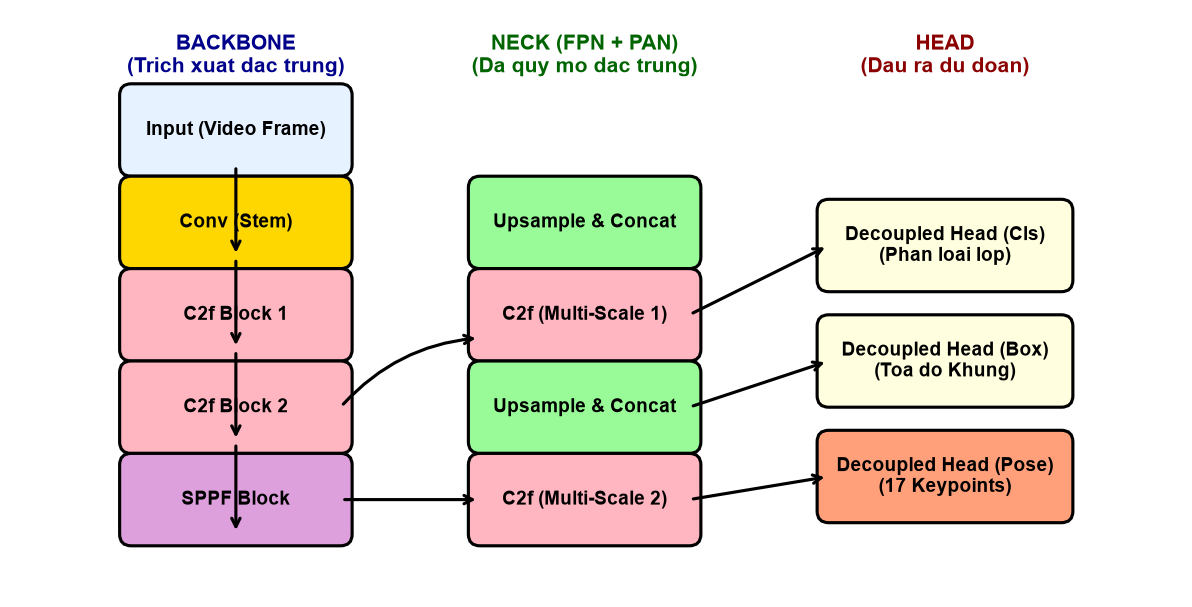
\includegraphics[width=0.95\textwidth]{Images/yolov8_architecture.png}
    \caption[Kiến trúc mạng nơ-ron tích chập YOLOv8]{\bfseries\fontsize{12pt}{0pt}\selectfont Kiến trúc mạng nơ-ron tích chập YOLOv8}
    \label{fig:yolov8_architecture}
\end{figure}

\begin{itemize}
    \item \textbf{Backbone (Mạng xương sống)}: Sử dụng kiến trúc CSPDarknet53 cải tiến, trong đó khối C3 (CSPLayer với 3 tích chập) ở các phiên bản trước được thay thế bằng khối C2f (CSPLayer với 2 tích chập nhanh). Khối C2f kết hợp các luồng đặc trưng cấp cao và cấp thấp, giúp tăng cường khả năng học biểu diễn đặc trưng đa quy mô và cải thiện dòng gradient lan truyền ngược mà không làm tăng kích thước mô hình.
    \item \textbf{Neck (Mạng cổ)}: Sử dụng cấu trúc PANet (Path Aggregation Network) kết hợp FPN (Feature Pyramid Network). Cấu trúc này giúp truyền dẫn thông tin đặc trưng ngữ cảnh từ các lớp sâu xuống các lớp nông và ngược lại. Điều này cực kỳ quan trọng đối với dữ liệu từ UAV, nơi kích thước của nạn nhân thay đổi liên tục theo độ cao bay.
    \item \textbf{Head (Đầu dự đoán)}: Điểm cải tiến cốt lõi của YOLOv8 là việc chuyển dịch từ kiến trúc dựa trên Anchor (Anchor-based) sang kiến trúc không dựa trên Anchor (Anchor-free/Anchor-less). Nhờ việc dự đoán trực tiếp tọa độ tâm và kích thước của đối tượng, mô hình giảm thiểu số lượng hộp neo cần tính toán trước, tăng tốc độ hội tụ và giảm độ phức tạp của hàm mất mát. Hơn nữa, YOLOv8 sử dụng cơ chế Decoupled Head, tách biệt nhánh dự đoán lớp (Classification) và dự đoán tọa độ (Regression), giúp nâng cao hiệu năng huấn luyện.
\end{itemize}

\subsubsection{Quy trình thu thập và tiền xử lý dữ liệu qua nền tảng Roboflow}

Nhằm đảm bảo tính hội tụ và độ chính xác của mô hình học sâu, tập dữ liệu huấn luyện cần được quản lý theo quy trình chuẩn hóa. Việc khai thác dữ liệu từ hệ sinh thái thị giác máy tính Roboflow Universe được triển khai qua các bước tiêu chuẩn như sau:

\begin{figure}[H]
    \centering
    
\includegraphics[width=0.85\textwidth]{Images/yolo_ai/roboflow_process.jpg}
    \caption[Quy trình tiền xử lý và tăng cường dữ liệu trên Roboflow]{\bfseries\fontsize{12pt}{0pt}\selectfont Quy trình tiền xử lý và tăng cường dữ liệu trên Roboflow}
    \label{fig:roboflow_process}
\end{figure}

\begin{itemize}
    \item \textbf{Thu thập dữ liệu}: Trích xuất các tập dữ liệu có độ phủ không gian lớn, đa dạng về bối cảnh, điều kiện ánh sáng và góc độ quan sát để tăng tính tổng quát hóa cho mô hình.
    \item \textbf{Tiền xử lý (Preprocessing)}: Đồng bộ hóa hình ảnh đầu vào, thực hiện điều chỉnh kích thước (resize) để tương thích với kiến trúc mạng YOLO (ví dụ: kích thước tiêu chuẩn $640 \times 640$ pixel).
    \item \textbf{Tăng cường dữ liệu (Data Augmentation)}: Áp dụng các phép biến đổi nhiễu động như xoay, lật hình ảnh, hoặc điều chỉnh độ sáng/độ tương phản. Kỹ thuật này mở rộng không gian mẫu hình học, giúp mô hình tăng cường khả năng kháng nhiễu và hạn chế hiện tượng học vẹt (overfitting).
    \item \textbf{Trích xuất và định dạng}: Kết xuất tập dữ liệu theo định dạng tương thích với framework YOLO. Bộ dữ liệu đầu ra bao gồm hình ảnh gốc, các tệp văn bản nhãn hóa tọa độ hộp giới hạn (bounding box), cùng tệp tin cấu hình môi trường định nghĩa rõ số lượng và tên các lớp (classes).
\end{itemize}

\subsubsection{Ứng dụng mô hình chuyên biệt YOLOv8-Rescue và YOLOv8-Posture}

Nhằm tối ưu hóa hiệu quả phát hiện nạn nhân trong môi trường thực tế phức tạp (chứa nhiều chướng ngại vật như cây cối, đổ nát, nguồn sáng phức tạp), đồ án phát triển hai mô hình chuyên biệt chạy song song trên máy trạm mặt đất:

\begin{enumerate}
    \item \textbf{Mô hình phát hiện nạn nhân (YOLOv8-Rescue)}: Được huấn luyện trên bộ dữ liệu tùy chỉnh chứa các nhãn đối tượng bao gồm: \textit{Human} (người bình thường), \textit{Victim} (nạn nhân gặp nạn), \textit{Life\_buoy} (phao cứu sinh) và \textit{Boat} (thuyền cứu hộ). Mô hình tập trung vào việc xác định vị trí và bounding box của đối tượng người trong bối cảnh cứu nạn cứu hộ.
    \item \textbf{Mô hình phân loại tư thế người (YOLOv8-Posture)}: Được tinh chỉnh (fine-tuned) để phân loại nhanh tư thế của đối tượng thành các trạng thái: \textit{Standing} (đứng), \textit{Sitting} (ngồi), \textit{Lying/Fallen} (nằm/ngã), và \textit{Collapsed} (gục, nghiêng người). Việc phân loại nhanh tư thế là tiền đề quan trọng để đánh giá mức độ khẩn cấp ban đầu.
\end{enumerate}

\subsection{Cấu trúc bộ dữ liệu huấn luyện}

Hiện tại, quá trình huấn luyện đang được tiến hành trên hai mô hình nhận diện chuyên biệt, sử dụng các tập dữ liệu đã được tổng hợp, gán nhãn và phân chia một cách có hệ thống.

\subsubsection{Tập dữ liệu Phát hiện Cứu hộ (YOLOv8-Rescue)}

Tổng khối lượng dữ liệu phục vụ bài toán phân loại và phát hiện trạng thái cứu hộ là 82.623 hình ảnh. Tập dữ liệu huấn luyện bao gồm 65.515 ảnh cung cấp các đặc trưng thị giác cốt lõi để mạng nơ-ron tối ưu hóa trọng số qua các vòng lặp. Tập kiểm thử bao gồm 10.173 ảnh độc lập được tách biệt hoàn toàn khỏi quá trình cập nhật trọng số để đánh giá khách quan hiệu năng mô hình. Cấu trúc phân vùng chi tiết của tập dữ liệu cứu hộ được tổng hợp trong Bảng \ref{tab:dataset_rescue}.

\begin{table}[H]
    \centering
    \caption[Phân vùng chi tiết tập dữ liệu huấn luyện YOLOv8-Rescue]{\bfseries\fontsize{12pt}{0pt}\selectfont Phân vùng chi tiết tập dữ liệu huấn luyện YOLOv8-Rescue}
    \begin{tabularx}{\textwidth}{|l|X|c|c|c|c|}
    \hline
    \rowcolor{LightCyan}
    \textbf{Mã DS} & \textbf{Tên tập dữ liệu gốc} & \textbf{Lớp gán} & \textbf{Ảnh Train} & \textbf{Ảnh Valid} & \textbf{Tổng cộng} \\ \hline
    ds0 & Disaster Victim v1 & 1 & 295 & 85 & 380 \\ \hline
    ds1 & Drowning Detection v1 & 0, 1 & 1.477 & 241 & 1.718 \\ \hline
    ds2 & Emergency Response v1 & 0, 1 & 1.958 & 302 & 2.260 \\ \hline
    ds3 & People Detection General & 0 & 13.449 & 2.133 & 15.582 \\ \hline
    ds4 & COCO Person v1 & 0 & 4.194 & 1.049 & 5.243 \\ \hline
    ds5 & Disaster for YOLO & 0 & 471 & 10 & 481 \\ \hline
    ds6 & Drone Person Detection & 0 & 1.870 & 274 & 2.144 \\ \hline
    ds7 & General Person Dataset & 0 & 2.314 & 997 & 3.311 \\ \hline
    ds8 & VisDrone2019 v3 & 0 & 3.946 & 481 & 4.427 \\ \hline
    ds9 & Injured People Detection & 1 & 112 & 26 & 138 \\ \hline
    ds10 & Injured People v1 & 0, 1 & 384 & 37 & 421 \\ \hline
    ds11 & People Detection Thermal & 0 & 21.422 & 3.061 & 24.483 \\ \hline
    ds13 & Rescue Dataset v1 & 1 & 405 & 38 & 443 \\ \hline
    ds14 & SOS Detection v1 & 0, 1 & 246 & 30 & 276 \\ \hline
    ds15 & Drowning Dataset v2 & 0, 1 & 8.284 & 804 & 9.088 \\ \hline
    ds16 & Rubble \& Person Detection & 0, 1 & 8.804 & 802 & 9.606 \\ \hline
    ds17 & Victim Detection v1 & 1 & 2.020 & 602 & 2.622 \\ \hline
    \end{tabularx}
    \label{tab:dataset_rescue}
\end{table}

\subsubsection{Tập dữ liệu Phân loại Tư thế (YOLOv8-Posture)}

Đối với bài toán nhận diện hành vi động học, mô hình sử dụng kho dữ liệu quy mô 19.523 hình ảnh. Tập huấn luyện chứa 16.637 ảnh chịu trách nhiệm huấn luyện mạng trích xuất đặc trưng hình thái của đối tượng ở ba trạng thái cơ bản: Đứng, Ngồi và Nằm. Tập kiểm thử bao gồm 2.886 ảnh được dùng để đo lường khách quan hiệu năng và kiểm soát hiện tượng quá khớp. Chi tiết cấu trúc tập dữ liệu tư thế được tổng hợp trong Bảng \ref{tab:dataset_posture}.

\begin{table}[H]
    \centering
    \caption[Phân vùng chi tiết tập dữ liệu huấn luyện YOLOv8-Posture]{\bfseries\fontsize{12pt}{0pt}\selectfont Phân vùng chi tiết tập dữ liệu huấn luyện YOLOv8-Posture}
    \begin{tabularx}{\textwidth}{|l|X|c|c|c|c|}
    \hline
    \rowcolor{LightCyan}
    \textbf{Mã DS} & \textbf{Tên tập dữ liệu gốc} & \textbf{Lớp gán} & \textbf{Ảnh Train} & \textbf{Ảnh Valid} & \textbf{Tổng cộng} \\ \hline
    dsA & Fall Detection v1 & 0, 1, 2 & 6.852 & 569 & 7.421 \\ \hline
    dsB & Fall Detection Raw & 2 & 3.148 & 1.349 & 4.497 \\ \hline
    dsC & Fall Down Detection & 0, 1, 2 & 3.500 & 750 & 4.250 \\ \hline
    dsE & Sitting Person v2 & 1 & 536 & 115 & 651 \\ \hline
    dsF & Person Standing & 0 & 195 & 40 & 235 \\ \hline
    dsG & Standing Person & 0 & 141 & 63 & 204 \\ \hline
    dsH & Standing Dataset & 0 & 91 & 0 & 91 \\ \hline
    dsI & Sitting Dataset & 1 & 2.174 & 0 & 2.174 \\ \hline
    \end{tabularx}
    \label{tab:dataset_posture}
\end{table}

\subsection{Ước lượng tư thế người (Pose Estimation) dựa trên YOLO-Pose}

Bên cạnh việc phát hiện bounding box, việc phân tích chi tiết tư thế hình học của cơ thể người đóng vai trò sống còn trong việc nhận diện nạn nhân đang gặp nguy hiểm (ví dụ: bị thương không thể đứng dậy, ngất xỉu). Đồ án sử dụng mô hình YOLOv8-Pose để ước lượng tư thế người thời gian thực.

\subsubsection{Nguyên lý ước lượng tư thế người và trích xuất 17 keypoints}

Mô hình YOLOv8-Pose thực hiện dự đoán đồng thời vị trí bounding box và tọa độ của 17 điểm mốc (keypoints) trên cơ thể người trong cùng một lượt quét (single-shot). Cấu trúc 17 keypoints tiêu chuẩn theo bộ dữ liệu COCO bao gồm các vị trí khớp xương chính trên cơ thể người, được minh họa trong Hình \ref{fig:yolo_pose_17_keypoints}.

\begin{figure}[H]
    \centering
    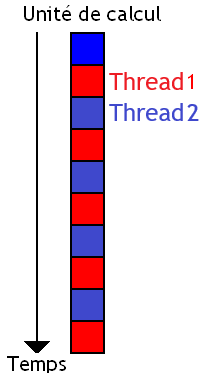
\includegraphics[width=0.55\textwidth]{Images/agent/yolo_pose_17_keypoints.png}
    \caption[Sơ đồ 17 điểm keypoints trên cơ thể người của YOLO-Pose]{\bfseries\fontsize{12pt}{0pt}\selectfont Sơ đồ 17 điểm keypoints trên cơ thể người của YOLO-Pose}
    \label{fig:yolo_pose_17_keypoints}
\end{figure}

Danh sách 17 điểm keypoints trích xuất từ mô hình bao gồm:
\begin{multicols}{2}
\begin{itemize}
    \item 0: Mũi (Nose)
    \item 1: Mắt trái (L-Eye), 2: Mắt phải (R-Eye)
    \item 3: Tai trái (L-Ear), 4: Tai phải (R-Ear)
    \item 5: Vai trái (L-Shoulder), 6: Vai phải (R-Shoulder)
    \item 7: Khuỷu tay trái (L-Elbow), 8: Khuỷu phải (R-Elbow)
    \item 9: Cổ tay trái (L-Wrist), 10: Cổ tay phải (R-Wrist)
    \item 11: Hông trái (L-Hip), 12: Hông phải (R-Hip)
    \item 13: Đầu gối trái (L-Knee), 14: Đầu gối phải (R-Knee)
    \item 15: Cổ chân trái (L-Ankle), 16: Cổ chân phải (R-Ankle)
\end{itemize}
\end{multicols}

\subsubsection{Phân tích hình học tư thế dựa trên tọa độ keypoints}

Dựa trên tọa độ pixel của 17 keypoints, thuật toán tiến hành phân tích các chỉ số hình học để tự động phát hiện trạng thái nằm/ngã (Fall/Lying detection) hoặc gục đổ (Collapsed):

\begin{itemize}
    \item \textbf{Tỷ lệ góc nghiêng thân người}: Chỉ số này được tính toán thông qua góc lệch của đường thẳng nối giữa trung điểm hai vai (trung bình cộng tọa độ vai trái và vai phải) và trung điểm hai hông (trung bình cộng tọa độ hông trái và hông phải) so với phương ngang của ảnh. Nếu góc nghiêng thân người nhỏ hơn một ngưỡng thiết lập thích hợp (cụ thể là dưới 35 độ), điều đó chứng tỏ thân người đang ở tư thế nằm ngang hoặc ngã trên mặt đất thay vì đứng thẳng (góc nghiêng thân người xấp xỉ 90 độ).
    \item \textbf{Tỷ lệ khung bao (Bounding Box Aspect Ratio)}: Định nghĩa bằng tỷ lệ giữa chiều rộng và chiều cao của hộp giới hạn bao quanh đối tượng. Đối với người đứng thẳng bình thường, chiều ngang nhỏ hơn nhiều so với chiều dọc nên tỷ lệ này thường nhỏ hơn 0.5. Khi đối tượng bị ngã hoặc nằm ra đất, chiều ngang hộp bao tăng lên rõ rệt và chiều cao giảm đi, làm tỷ lệ khung bao tăng mạnh vượt ngưỡng 1.2.
\end{itemize}

Sự kết hợp đồng thời giữa điều kiện góc nghiêng thân người nhỏ hơn 35 độ và tỷ lệ khung bao lớn hơn 1.2 cấu thành dấu hiệu hình học chắc chắn để xác định trạng thái nằm/ngã của nạn nhân với độ tin cậy cao mà không cần dựa vào các phép toán phức tạp.

\subsection{Thuật toán phân tích cử chỉ động và trạng thái nạn nhân}

Trong công tác tìm kiếm cứu hộ thực tế, nạn nhân thường cố gắng phát tín hiệu cầu cứu tới các thiết bị bay bằng cách vẫy tay. Đồng thời, những nạn nhân bị bất tỉnh sẽ nằm bất động hoàn toàn. Do đó, việc phân tích cử chỉ động theo thời gian là vô cùng cần thiết.

\subsubsection{Phát hiện cử chỉ vẫy hai tay cầu cứu (two\_hands\_waving)}

Cử chỉ vẫy hai tay cầu cứu được định nghĩa động học là sự di chuyển tuần hoàn của hai cổ tay lên phía trên đường nối hai vai theo phương dọc và có sự dao động qua lại theo phương ngang. Thuật toán lưu trữ chuỗi thời gian tọa độ của 30 khung hình gần nhất (tương đương khoảng 1.2 giây ở tốc độ xử lý 25 FPS). Quy trình phát hiện bao gồm các bước sau:

\begin{enumerate}
    \item \textbf{Chuẩn hóa tọa độ}: Để thuật toán hoạt động ổn định và độc lập với khoảng cách từ Drone đến đối tượng, tọa độ dọc của cổ tay được chuẩn hóa bằng cách lấy khoảng cách dọc từ cổ tay đến vai chia cho chiều dài thân người (khoảng cách Euclid giữa vai và hông).
    \item \textbf{Kiểm tra điều kiện biên}: Cả hai cổ tay phải nằm phía trên vai. Trong hệ tọa độ ảnh gốc (với trục dọc hướng xuống dưới), điều này tương đương với việc trị số tọa độ dọc của các cổ tay nhỏ hơn tọa độ dọc của vai tương ứng.
    \item \textbf{Phân tích tần số dao động}: Tính toán độ biến động (độ lệch chuẩn) và số lần đổi hướng chuyển động theo phương ngang của hai cổ tay trong cửa sổ thời gian. Nếu số lần đổi hướng dọc theo trục ngang vượt quá 3 lần trong cửa sổ thời gian, đồng thời biên độ dao động ngang vượt qua một ngưỡng quy định, hệ thống sẽ xác nhận có chuyển động vẫy tay.
\end{enumerate}

Nếu các điều kiện chuẩn hóa và dao động trên đồng thời được thỏa mãn trong 3 chu kỳ liên tiếp, hệ thống xác nhận nạn nhân đang thực hiện cử chỉ "Vẫy hai tay cầu cứu".

\subsubsection{Thuật toán đánh giá trạng thái bất động tĩnh (immobility)}

Đối với các nạn nhân bị chấn thương nặng hoặc bất tỉnh, trạng thái bất động tĩnh kéo dài là dấu hiệu cực kỳ nguy cấp. Thuật toán giám sát sự bất động dựa trên biến động vị trí tâm mục tiêu (Centroid) theo thời gian.

Trọng tâm mục tiêu được tính bằng trung điểm tọa độ hộp bao. Hệ thống duy trì một hàng đợi chứa các vị trí trọng tâm trong khoảng thời gian quan sát 10 giây. Độ lệch tâm tích lũy được tính bằng độ biến động (độ lệch chuẩn tổng hợp) của các tọa độ trọng tâm trong hàng đợi.

Để loại bỏ ảnh hưởng do Drone bị rung lắc hoặc di chuyển dịch chuyển camera, tọa độ trọng tâm được bù trừ dựa trên véc-tơ chuyển động nền của toàn cảnh. Véc-tơ nền này được ước lượng bằng cách tính toán dòng quang học trên các điểm đặc trưng tĩnh của mặt đất. Nếu sau khoảng thời gian quan sát, độ lệch tâm sau khi bù trừ nhỏ hơn một ngưỡng động rất nhỏ (được điều chỉnh tự động theo độ cao bay của Drone), đồng thời mô hình phân loại tư thế xác nhận đối tượng đang ở tư thế nằm, hệ thống sẽ kích hoạt trạng thái "Bất động tĩnh khẩn cấp".

\subsection{Cơ chế dung hợp quyết định (Decision Fusion) đa mô hình}

Việc chỉ sử dụng đơn lẻ một mô hình học sâu rất dễ dẫn đến hiện tượng báo động giả (false alarm). Ví dụ, một người đang nằm ngủ bình thường trên bãi cỏ hoặc một hình nhân có thể bị mô hình YOLOv8-Rescue nhận diện nhầm là nạn nhân cứu hộ. Do đó, đồ án đề xuất cơ chế dung hợp quyết định đa nguồn ở mức suy luận (inference level). Sơ đồ luồng dung hợp được thể hiện trong Hình \ref{fig:decision_fusion_flow}.

\begin{figure}[H]
    \centering
    
\includegraphics[width=0.85\textwidth]{Images/anh_cho.png}
    \caption[Sơ đồ kiến trúc dung hợp quyết định đa luồng phân tích nạn nhân]{\bfseries\fontsize{12pt}{0pt}\selectfont Sơ đồ kiến trúc dung hợp quyết định đa luồng phân tích nạn nhân}
    \label{fig:decision_fusion_flow}
\end{figure}

\subsubsection{Thuật toán dung hợp tích lũy bằng chứng xác suất nạn nhân}

Hệ thống kết hợp ba nguồn thông tin độc lập thông qua mô hình trung bình trọng số: độ tin cậy phát hiện người ($C_{rescue}$ từ YOLOv8-Rescue), xác suất phân loại tư thế nằm ngã ($P_{lying}$ từ YOLOv8-Posture) và kết quả phân tích hình học từ YOLO-Pose ($P_{pose}$).

Xác suất nạn nhân thực sự cần cứu hộ $P(Victim)$ được tính bằng tổng có trọng số của ba thông số trên. Các hệ số trọng số được tối ưu hóa qua thực nghiệm trên tập dữ liệu thử nghiệm nhằm tối đa hóa F1-score, cụ thể được thiết lập là: trọng số của mô hình phát hiện cứu hộ chiếm 0.4, mô hình phân loại tư thế chiếm 0.3, và mô hình phân tích hình học tư thế chiếm 0.3. Tổng các hệ số trọng số này luôn bảo toàn bằng 1.0 để đảm bảo xác suất đầu ra chuẩn hóa từ 0 đến 1.

\subsubsection{Thiết lập hệ thống điểm nguy cấp Danger Score}

Để trạm mặt đất có thể tự động phân loại mức độ ưu tiên cứu hộ khi có nhiều mục tiêu xuất hiện cùng lúc trên màn hình giám sát, đồ án thiết lập hệ thống điểm nguy cấp (Danger Score - $DS$) chạy từ 0 đến 100 điểm.

Công thức tính Danger Score dựa trên xác suất xác nhận nạn nhân thực tế nhân với hệ số 50, cộng thêm điểm cộng hành vi động và điểm tích lũy theo thời gian bất động tĩnh. Điểm cộng hành vi được quy định: vẫy hai tay cầu cứu cộng 30 điểm; nằm bất động cộng 40 điểm; đứng hoặc đi lại bình thường cộng 0 điểm. Điểm tích lũy thời gian bất động tăng dần theo thời gian bất động tính bằng giây chia cho 3 và giới hạn tối đa 10 điểm.

Dựa trên trị số Danger Score thu được, hệ thống tự động phân loại cảnh báo theo các cấp độ quy tắc được định nghĩa trong Bảng \ref{tab:danger_rules}.

\begin{table}[H]
    \centering
    \caption[Bảng quy tắc phân loại trạng thái cứu hộ dựa trên Danger Score]{\bfseries\fontsize{12pt}{0pt}\selectfont Bảng quy tắc phân loại trạng thái cứu hộ dựa trên Danger Score}
    \begin{tabularx}{\textwidth}{|>{\centering\arraybackslash}m{2.2cm}|>{\centering\arraybackslash}m{2.5cm}|X|X|}
    \hline
    \rowcolor{LightCyan}
    \textbf{Ngưỡng điểm DS} & \textbf{Cấp độ cảnh báo} & \textbf{Mô tả trạng thái thực tế} & \textbf{Hành động của trạm} \\ \hline
    $DS < 40$ & Bình thường (Normal) & Đối tượng di chuyển ổn định, tư thế đứng/ngồi bình thường, không có dấu hiệu khẩn cấp. & Ghi log định kỳ, không cảnh báo. \\ \hline
    $40 \le DS < 75$ & Nghi ngờ (Suspicious) & Đối tượng nằm bất động thời gian ngắn dưới 5 giây hoặc có cử chỉ lạ chưa rõ ràng. & Đổi màu khung bao sang Vàng, tăng tần số trích xuất đặc trưng. \\ \hline
    $DS \ge 75$ & Cứu trợ khẩn cấp (Danger) & Đối tượng nằm bất động kéo dài hoặc vẫy tay cầu cứu liên tục, xác suất nạn nhân cao. & Đổi màu khung bao sang Đỏ, phát âm thanh báo động, chụp ảnh lưu trữ và xuất sự kiện. \\ \hline
    \end{tabularx}
    \label{tab:danger_rules}
\end{table}

Cơ chế này đảm bảo rằng các trường hợp nạn nhân bị bất tỉnh (đạt điểm Danger Score tối đa do cộng thêm điểm bất động kéo dài) hoặc nạn nhân đang tích cực vẫy tay cầu cứu sẽ ngay lập tức được đẩy lên mức ưu tiên cao nhất, giúp tối ưu hóa thời gian vàng trong công tác tìm kiếm cứu nạn.

\subsection{Đánh giá hiệu năng huấn luyện các mô hình YOLO}

Để minh chứng cho độ tin cậy và khả năng hội tụ của các thuật toán nhận dạng được nhúng trên trạm mặt đất, hiệu năng huấn luyện của hai mô hình YOLOv8-Posture và YOLOv8-Rescue qua 50 Epochs được theo dõi và phân tích chi tiết.

\subsubsection{Đánh giá hiệu năng mô hình phân tích tư thế (YOLOv8-Posture)}

\paragraph{Phân tích dữ liệu đầu vào (Data Distribution):}
Dựa trên thống kê từ tập dữ liệu huấn luyện cho bài toán nhận diện ba trạng thái tư thế, hệ thống ghi nhận sự phân bổ không đồng đều về mặt số lượng (Class Imbalance) giữa các lớp đối tượng, thể hiện trong Hình \ref{fig:posture_data_dist}.

\begin{figure}[H]
    \centering
    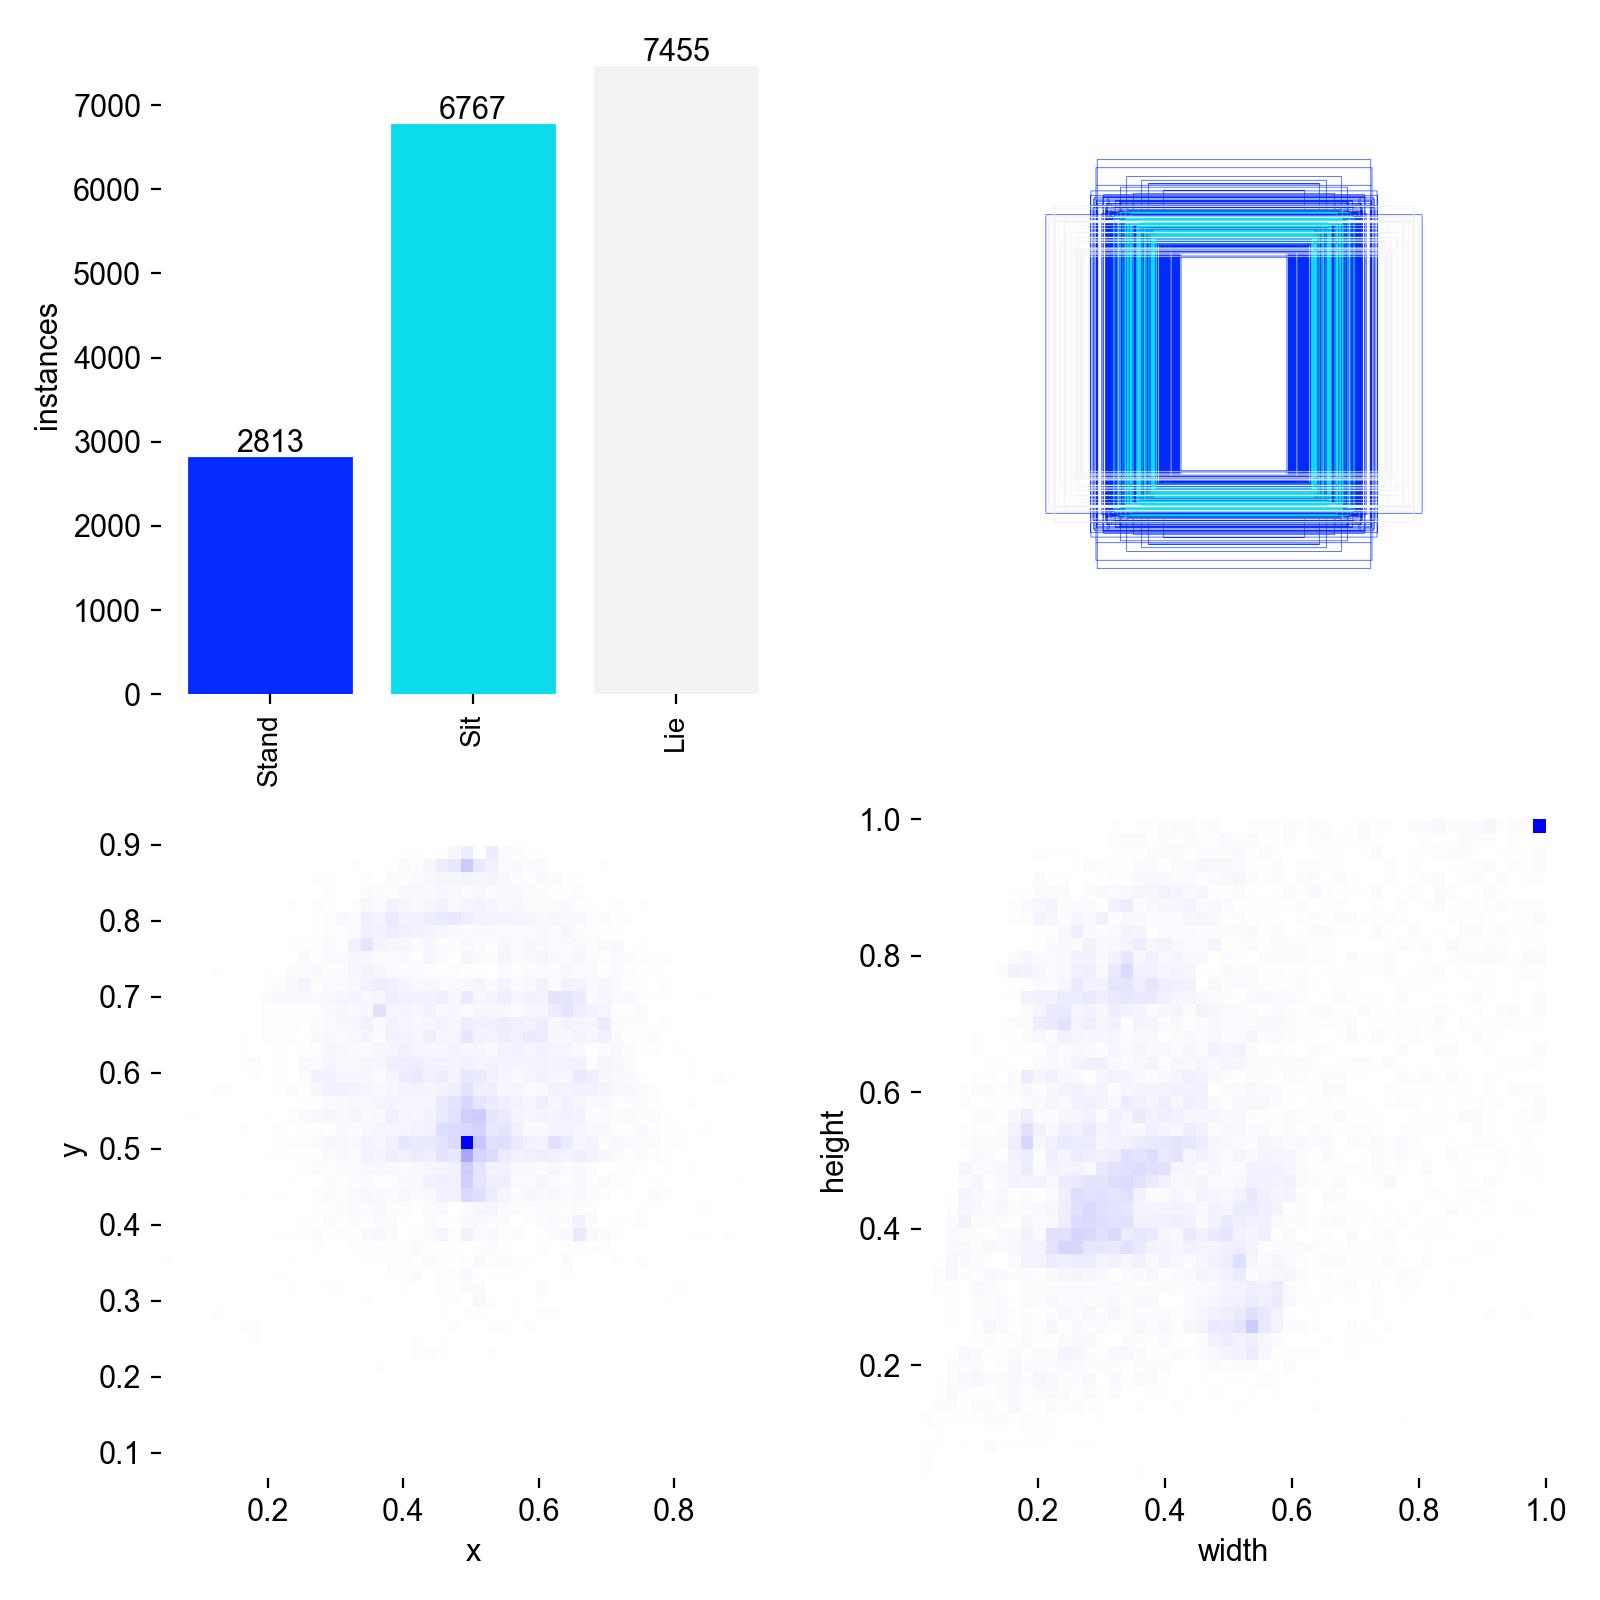
\includegraphics[width=0.65\textwidth]{Images/yolo_ai/posture_data_dist.png}
    \caption[Biểu đồ thống kê phân bổ số lượng khung giới hạn theo từng lớp tư thế]{\bfseries\fontsize{12pt}{0pt}\selectfont Biểu đồ thống kê phân bổ số lượng khung giới hạn theo từng lớp tư thế}
    \label{fig:posture_data_dist}
\end{figure}

Lớp tư thế Nằm (Lie) chiếm tỷ trọng đa số với 7.455 khung giới hạn, tiếp theo là lớp Ngồi (Sit) với 6.767 khung giới hạn, và lớp Đứng (Stand) có số lượng mẫu hạn chế nhất với 2.813 khung giới hạn. Sự chênh lệch này giải thích cho độ lệch biên trong kết quả phân loại đối với từng tư thế cụ thể của mô hình.

\paragraph{Đánh giá quá trình hội tụ (Model Convergence):}
Quá trình tối ưu hóa trọng số của mạng YOLOv8-Posture qua 50 Epochs phản ánh quỹ đạo hội tụ ổn định, thể hiện trong Hình \ref{fig:posture_loss}.

\begin{figure}[H]
    \centering
    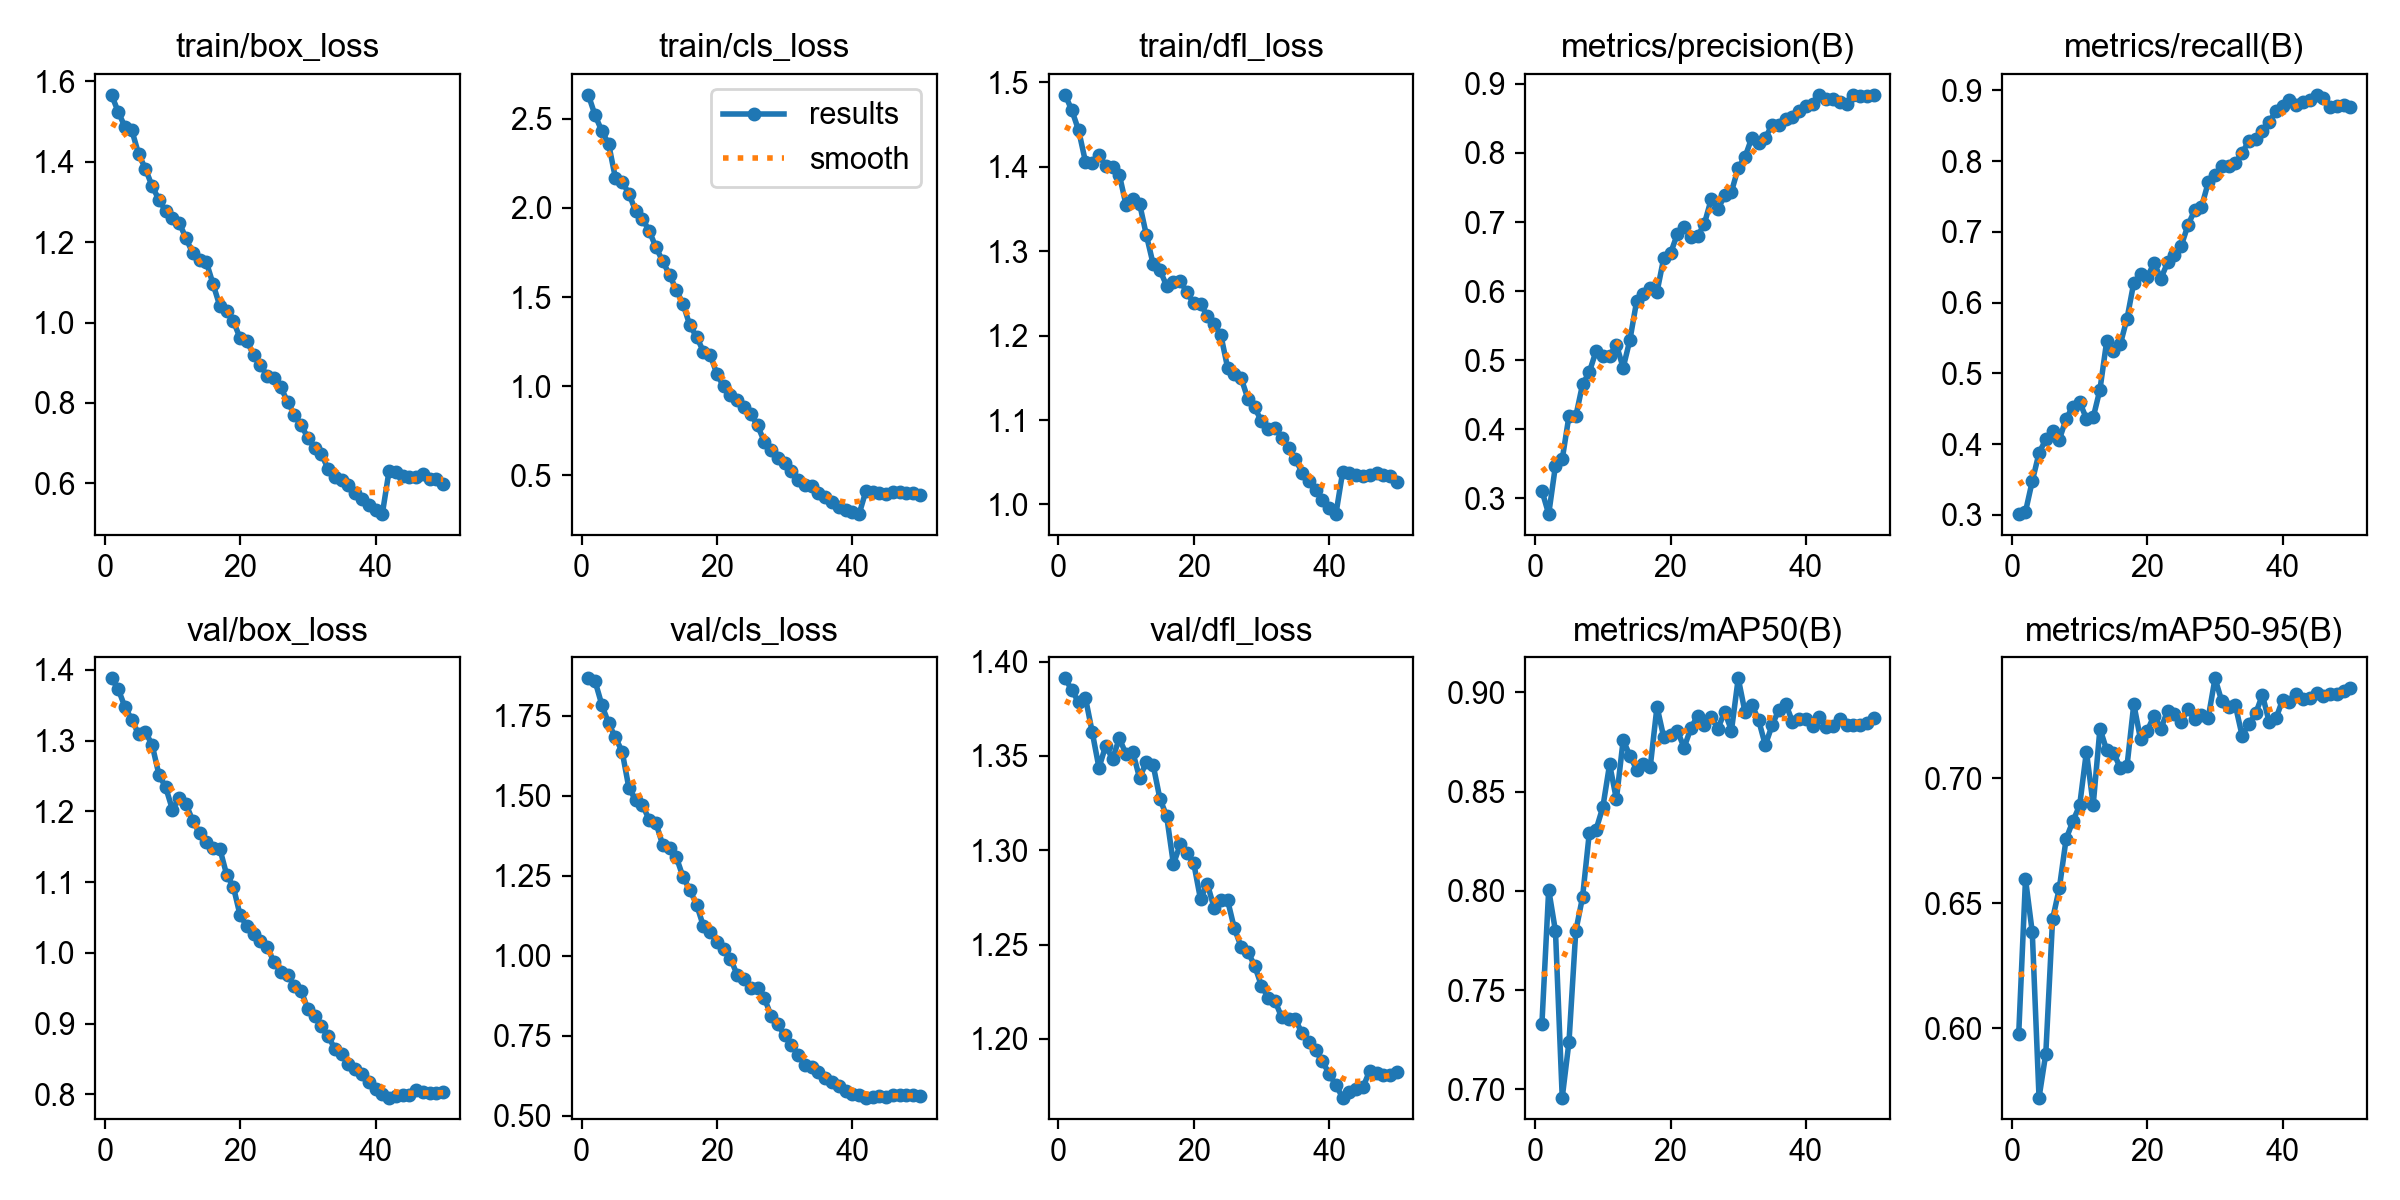
\includegraphics[width=0.75\textwidth]{Images/yolo_ai/posture_loss.png}
    \caption[Đồ thị biểu diễn hàm suy hao và chỉ số hiệu năng mô hình tư thế qua 50 Epochs]{\bfseries\fontsize{12pt}{0pt}\selectfont Đồ thị biểu diễn hàm suy hao và chỉ số hiệu năng mô hình tư thế qua 50 Epochs}
    \label{fig:posture_loss}
\end{figure}

Đường cong biểu diễn hàm suy hao trên tập huấn luyện (bao gồm box\_loss và cls\_loss) duy trì đà giảm mượt mà. Tại Epoch 50, hệ số mất mát trên tập dữ liệu kiểm thử (Validation) đạt mức tối ưu với val/box\_loss ghi nhận ở mức 0.79876 và val/cls\_loss đạt 0.56278. Sự suy giảm đồng thời giữa giá trị Train Loss và Validation Loss minh chứng năng lực tổng quát hóa tốt của mô hình, không xuất hiện trạng thái quá khớp.

\paragraph{Phân tích hiệu năng tổng thể (Overall Performance):}
Thông số kỹ thuật tại Epoch 50 chỉ ra năng lực dự báo cao của mạng nhận diện tư thế. Độ chính xác trung bình mAP@0.5 đạt mức cao 88.7\% (0.88701) và mAP@0.5:0.95 ổn định tại 73.64\% (0.73638).

\begin{figure}[H]
    \centering
    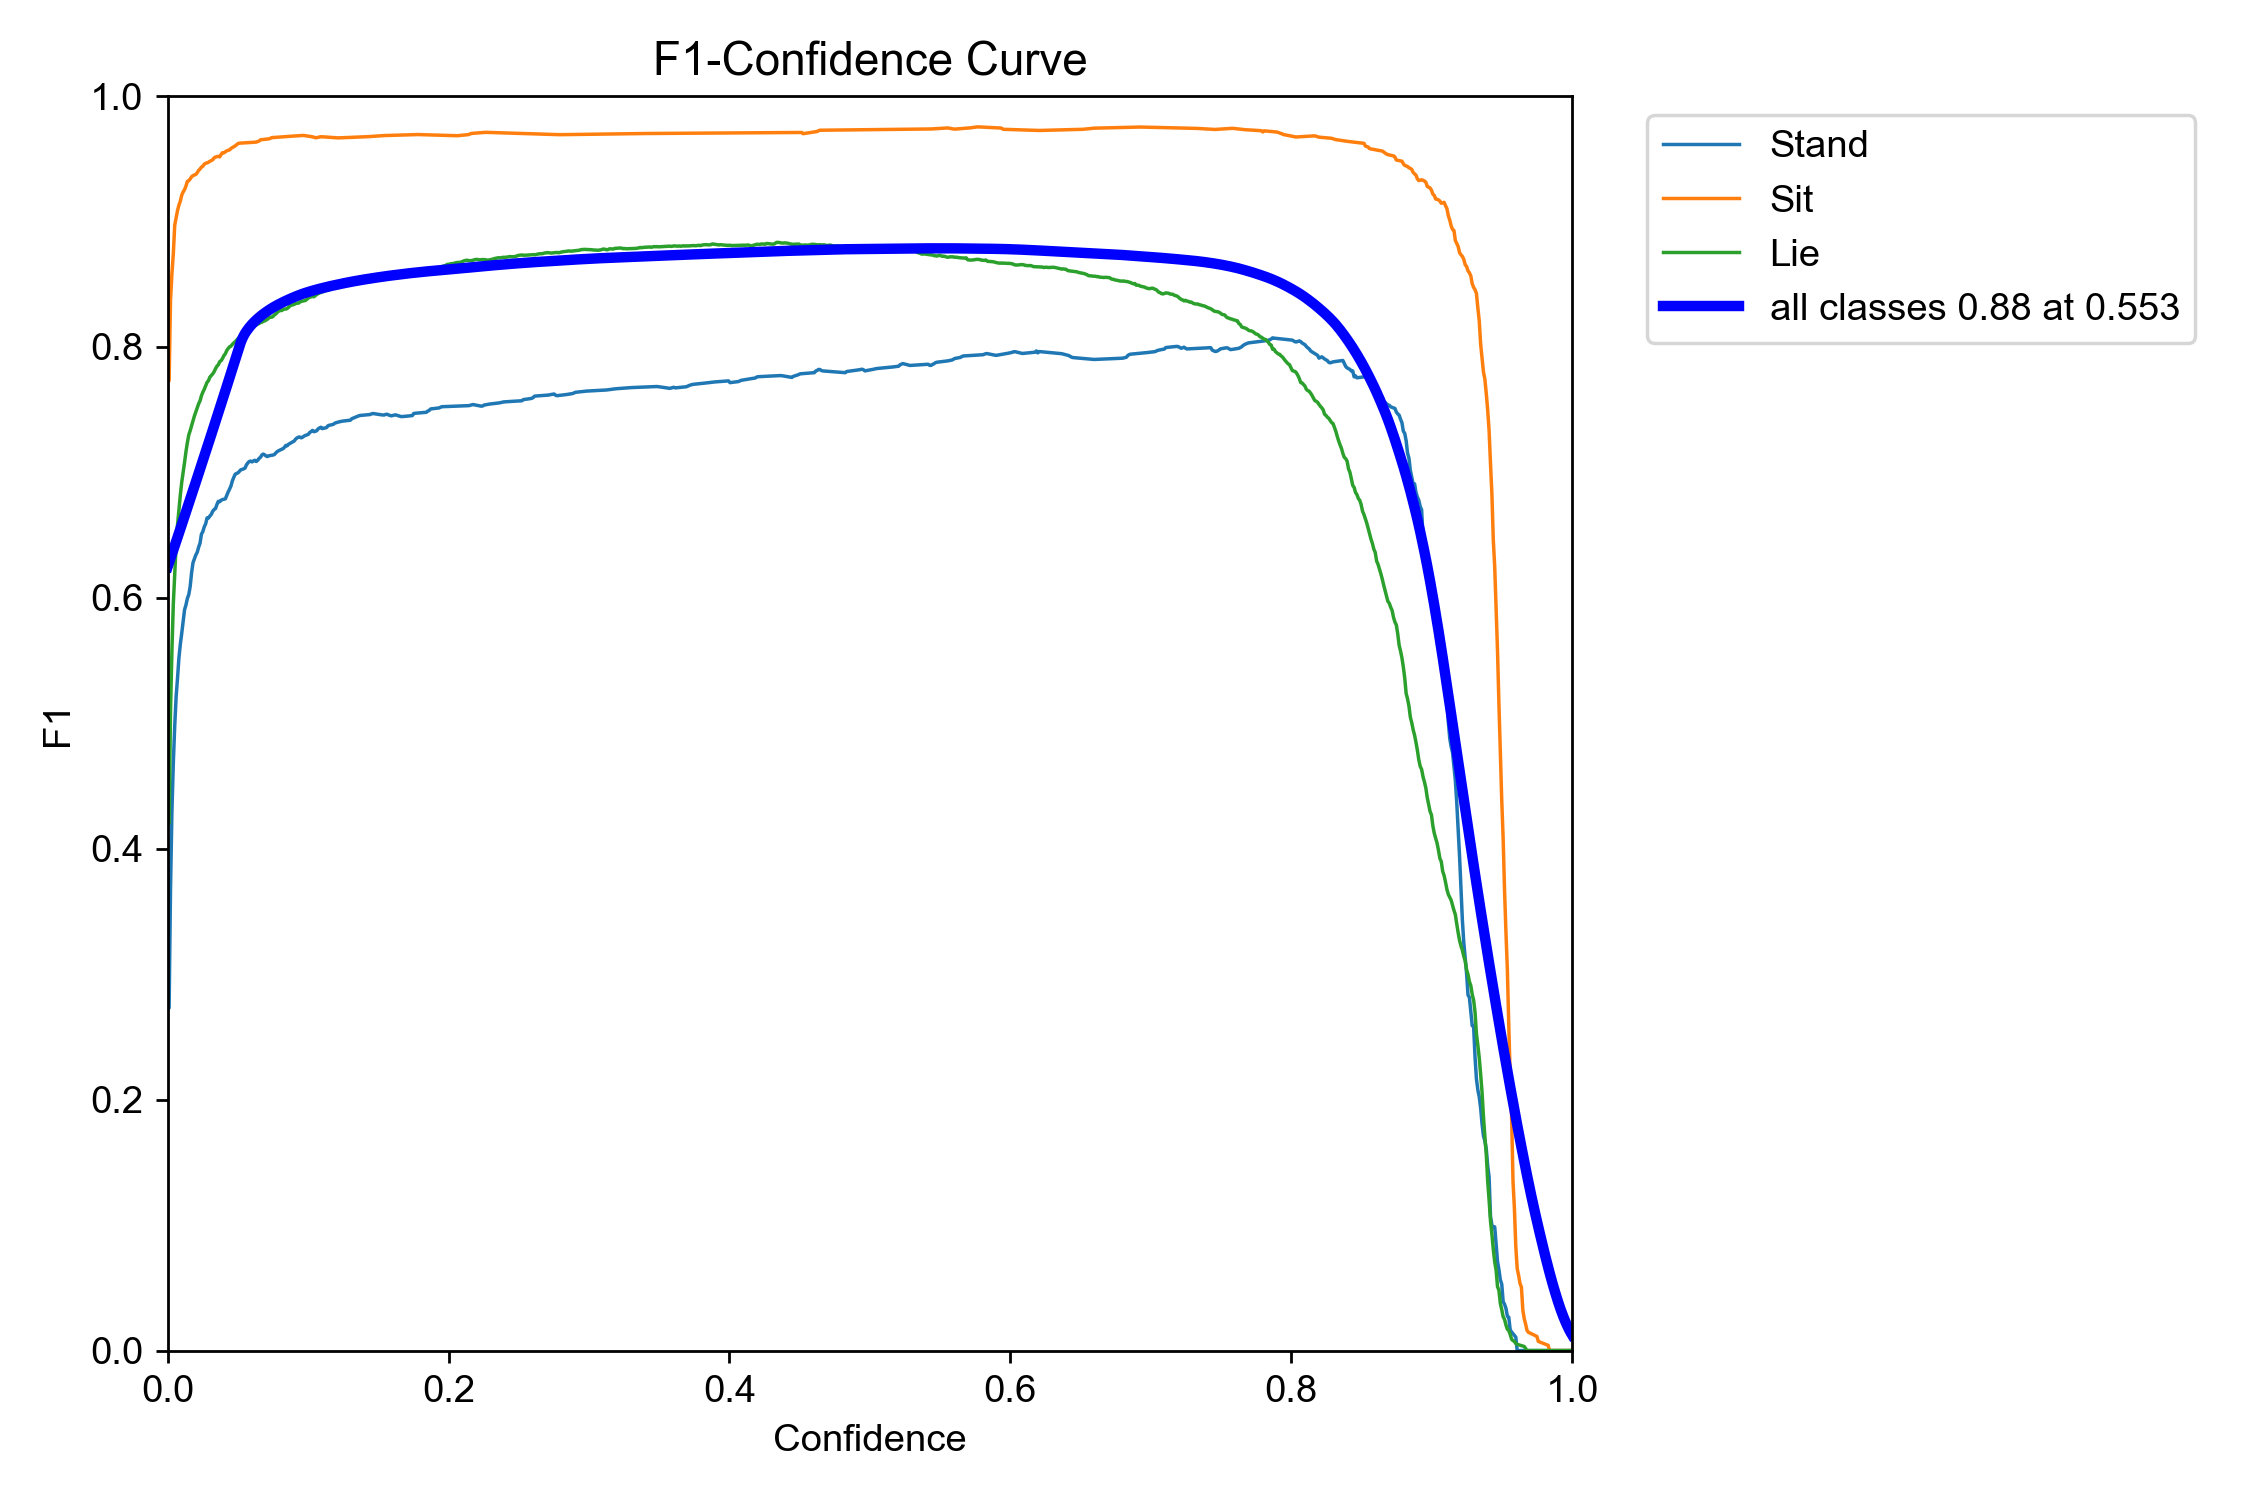
\includegraphics[width=0.65\textwidth]{Images/yolo_ai/posture_f1_curve.png}
    \caption[Đường cong F1-Confidence đánh giá sự cân bằng của mô hình tư thế]{\bfseries\fontsize{12pt}{0pt}\selectfont Đường cong F1-Confidence đánh giá sự cân bằng của mô hình tư thế}
    \label{fig:posture_f1_curve}
\end{figure}

Căn cứ trên phân tích đồ thị F1-Confidence ở Hình \ref{fig:posture_f1_curve}, chỉ số F1 tổng hợp đạt đỉnh (0.88) khi ngưỡng tin cậy (Confidence Threshold) được thiết lập tại 0.553. Đây là mức cài đặt tham chiếu khi triển khai thực tế trên máy trạm để cân bằng tối ưu giữa việc xuất hiện cảnh báo giả và việc bỏ sót mục tiêu.

\paragraph{Đánh giá độ nhạy cảm theo phân lớp (Class-Specific Performance):}
Độ nhạy cảm của thuật toán phân hóa rõ rệt đối với đặc trưng thị giác của từng lớp mục tiêu, được minh họa qua đường cong Precision-Recall ở Hình \ref{fig:posture_pr_curve} và ma trận nhầm lẫn ở Hình \ref{fig:posture_confusion_matrix}.

\begin{figure}[H]
    \centering
    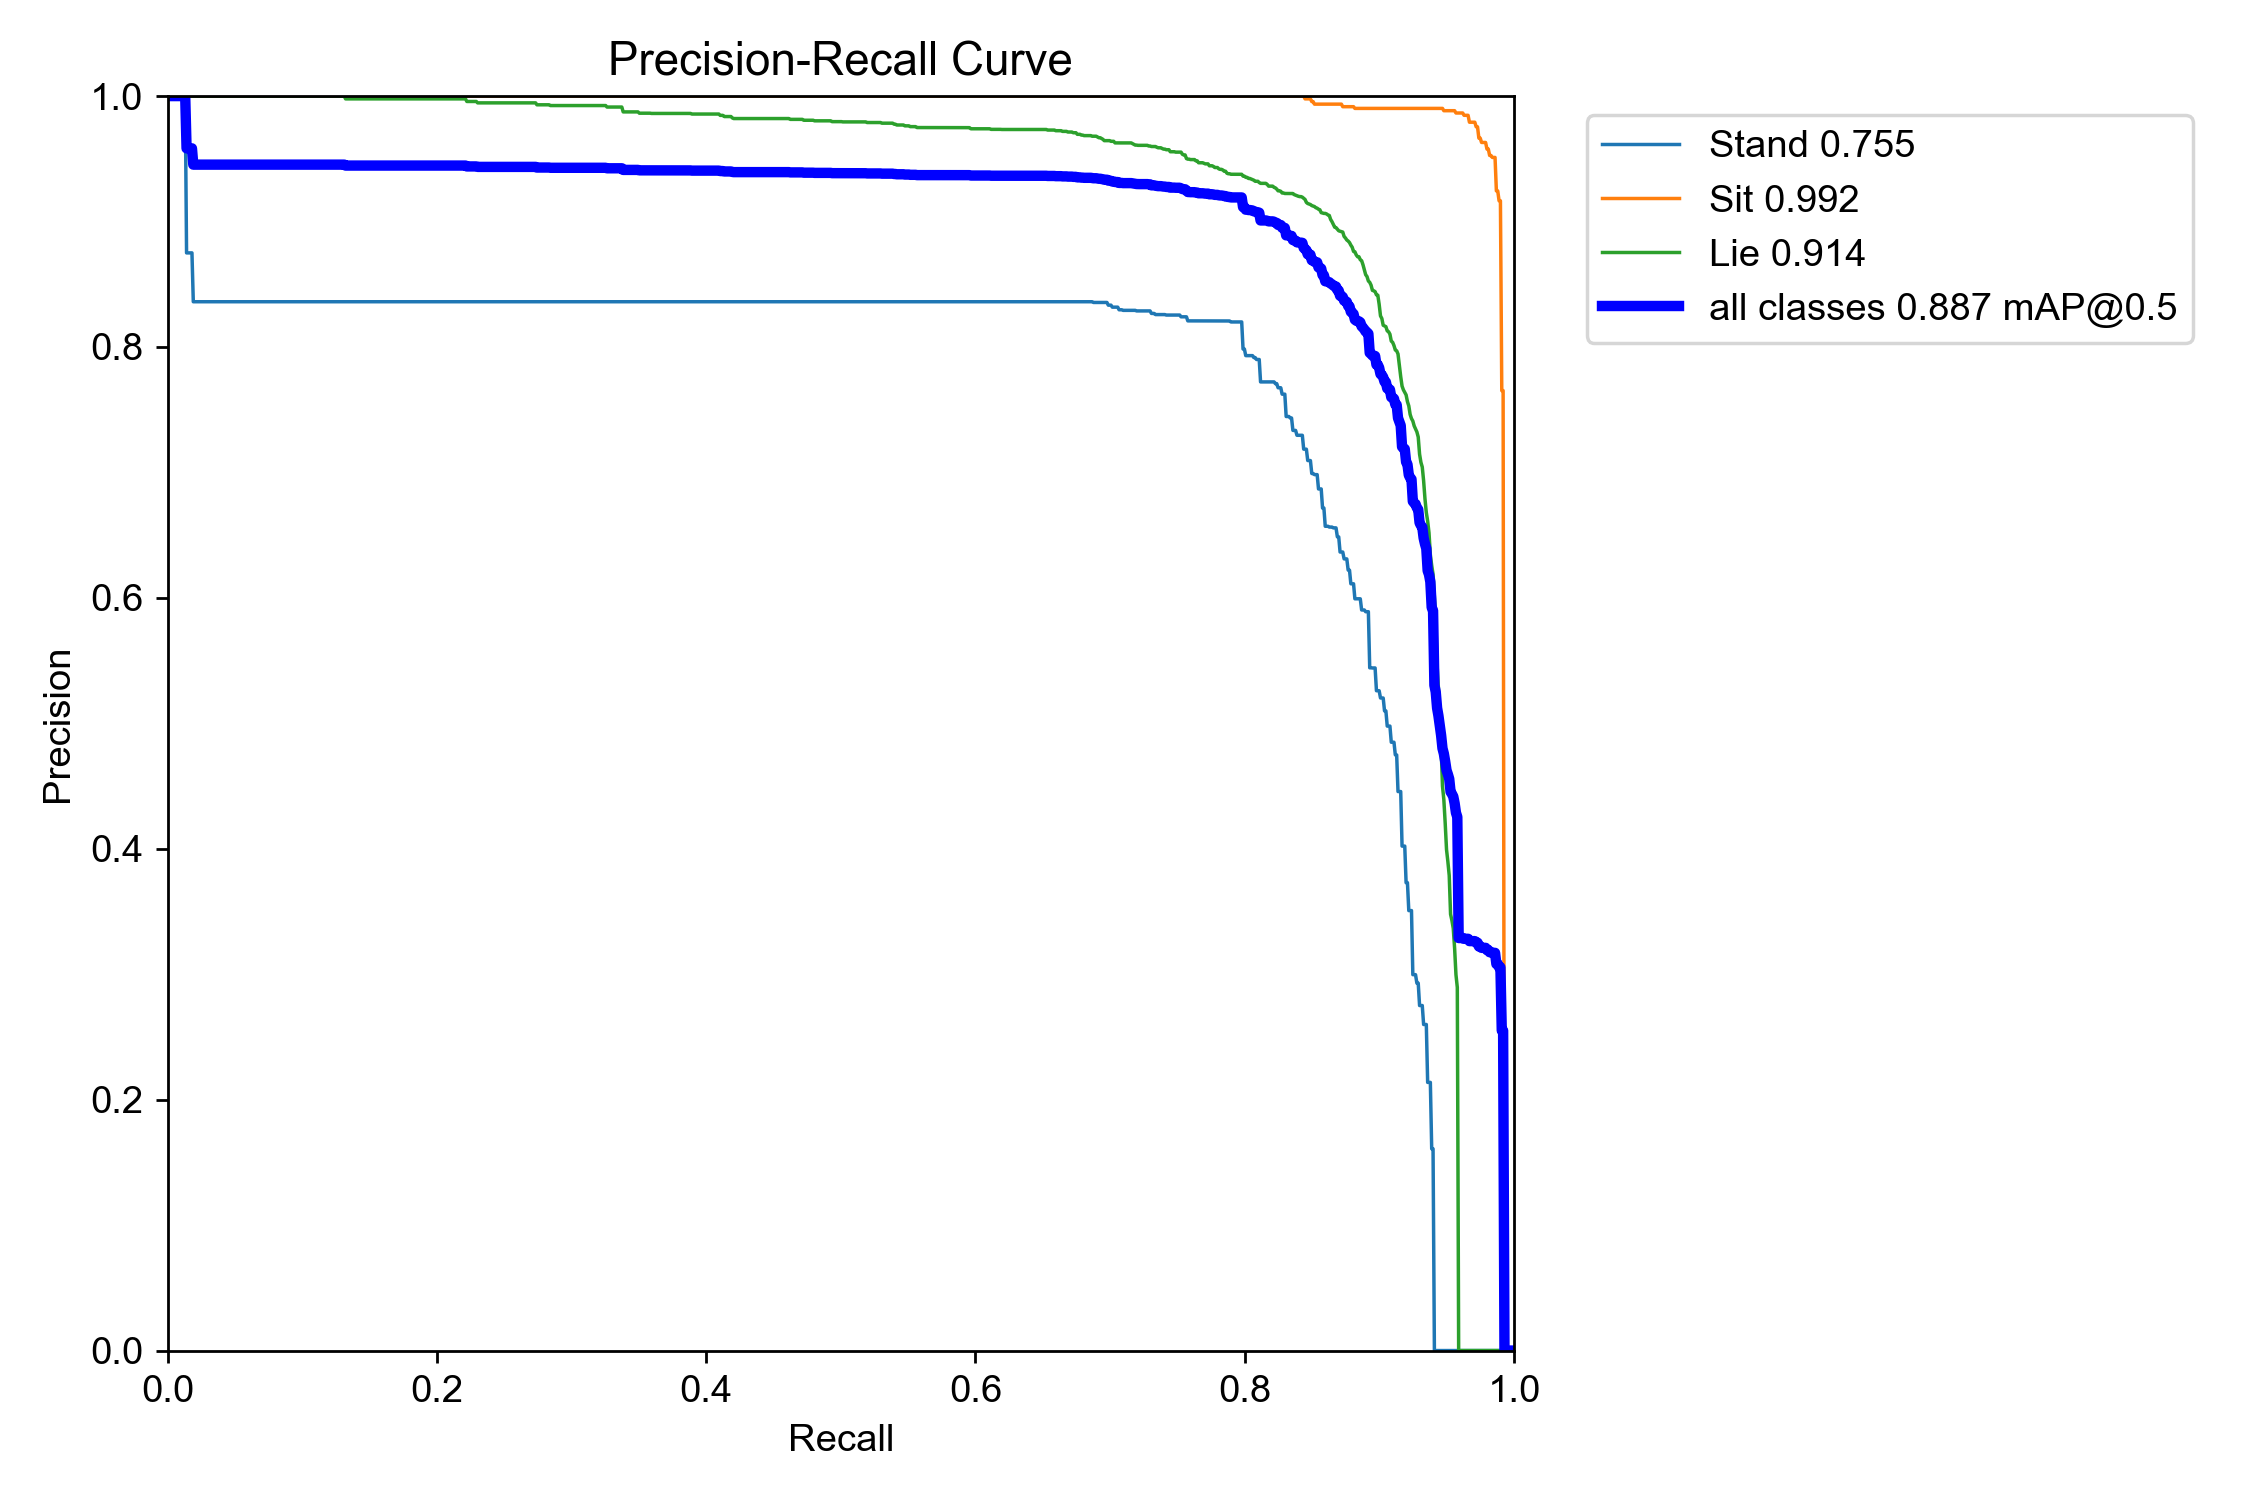
\includegraphics[width=0.65\textwidth]{Images/yolo_ai/posture_pr_curve.png}
    \caption[Đường cong Precision-Recall theo từng lớp tư thế]{\bfseries\fontsize{12pt}{0pt}\selectfont Đường cong Precision-Recall theo từng lớp tư thế}
    \label{fig:posture_pr_curve}
\end{figure}

\begin{figure}[H]
    \centering
    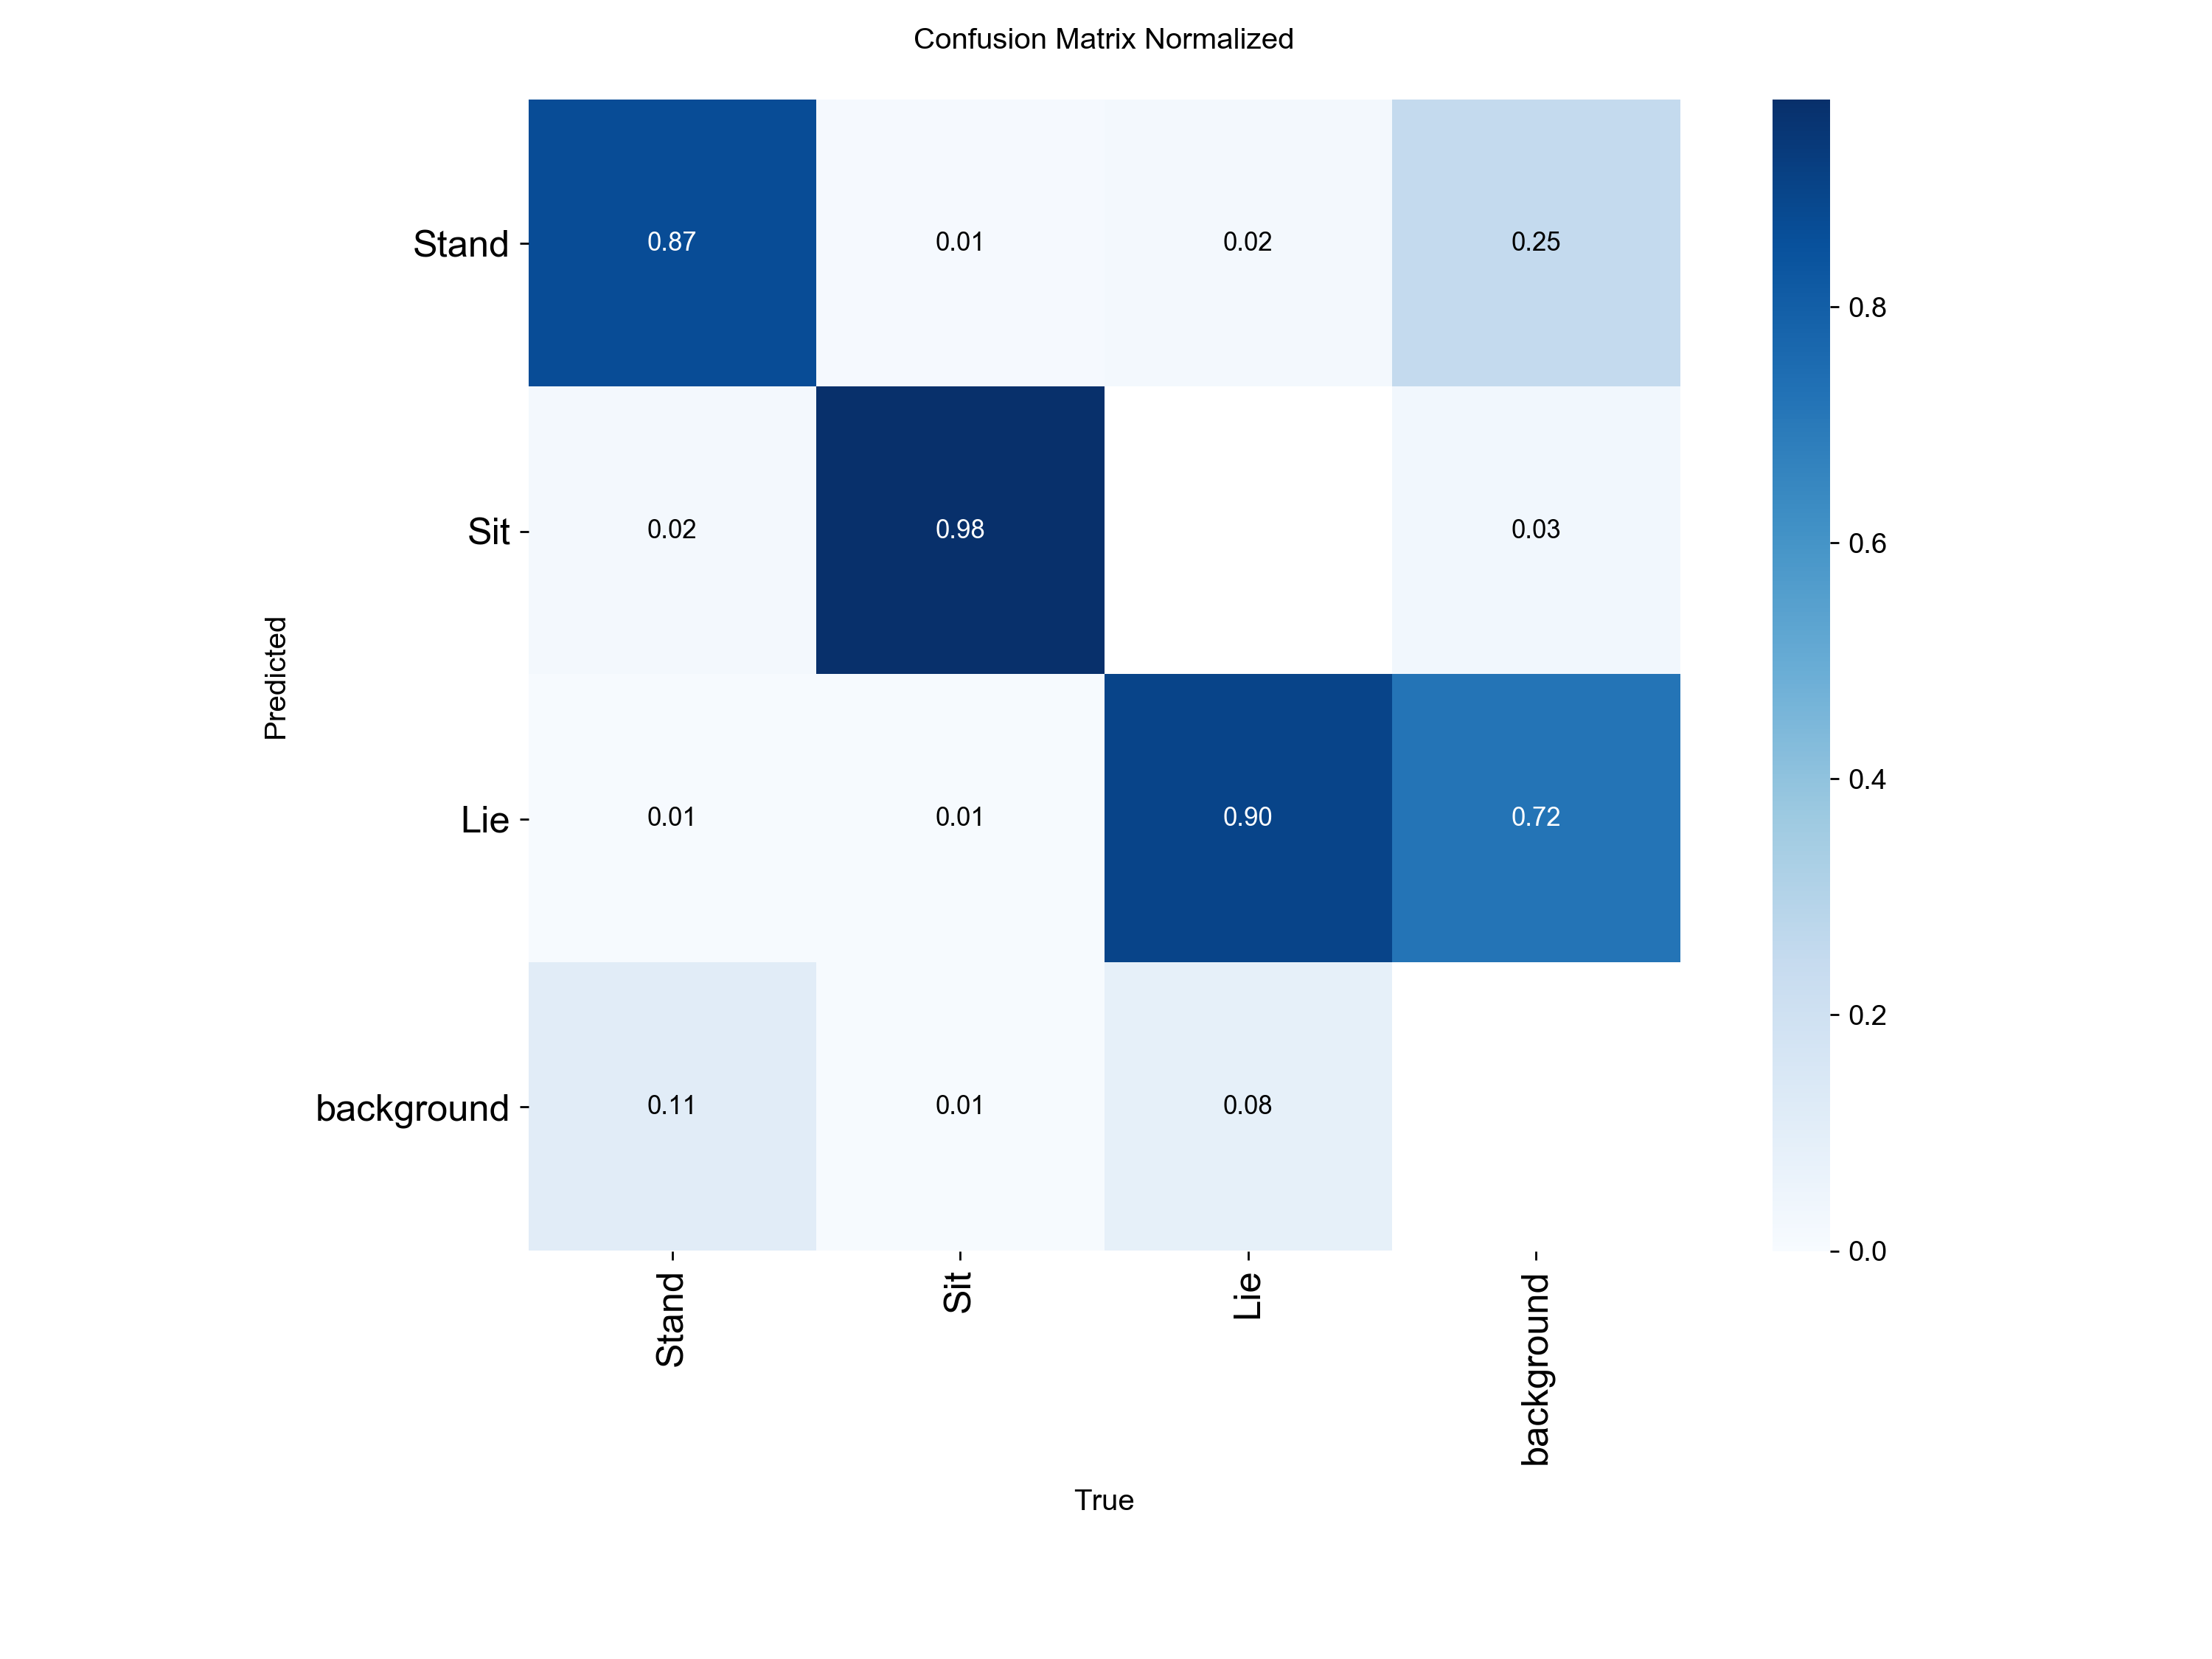
\includegraphics[width=0.6\textwidth]{Images/yolo_ai/posture_confusion_matrix.png}
    \caption[Ma trận nhầm lẫn chuẩn hóa của mô hình phân loại tư thế]{\bfseries\fontsize{12pt}{0pt}\selectfont Ma trận nhầm lẫn chuẩn hóa của mô hình phân loại tư thế}
    \label{fig:posture_confusion_matrix}
\end{figure}

Hành vi Ngồi (Sit) có khả năng nhận diện xuất sắc nhất với mAP@0.5 đạt 0.992 và tỷ lệ dự báo chính xác trong ma trận nhầm lẫn đạt 98\%. Tư thế Nằm (Lie) duy trì hiệu năng cao với chỉ số mAP@0.5 là 0.914, tỷ lệ chẩn đoán đúng đạt 90\% (khoảng 8\% bị nhầm thành nền). Tư thế Đứng (Stand) ghi nhận hiệu năng thấp nhất với mAP@0.5 ở mức 0.755 và tỷ lệ dự báo đúng đạt 87\% do số lượng mẫu huấn luyện hạn chế.

\subsubsection{Đánh giá hiệu năng mô hình phân tích cứu hộ (YOLOv8-Rescue)}

\paragraph{Phân bố dữ liệu đầu vào (Data Distribution):}
Dựa trên phân tích tập dữ liệu huấn luyện cho bài toán nhận diện trạng thái cứu hộ, hệ thống ghi nhận sự mất cân bằng dữ liệu cực kỳ lớn (Extreme Class Imbalance) giữa lớp người bình thường và nạn nhân gặp nạn, thể hiện trong Hình \ref{fig:rescue_data_dist}.

\begin{figure}[H]
    \centering
    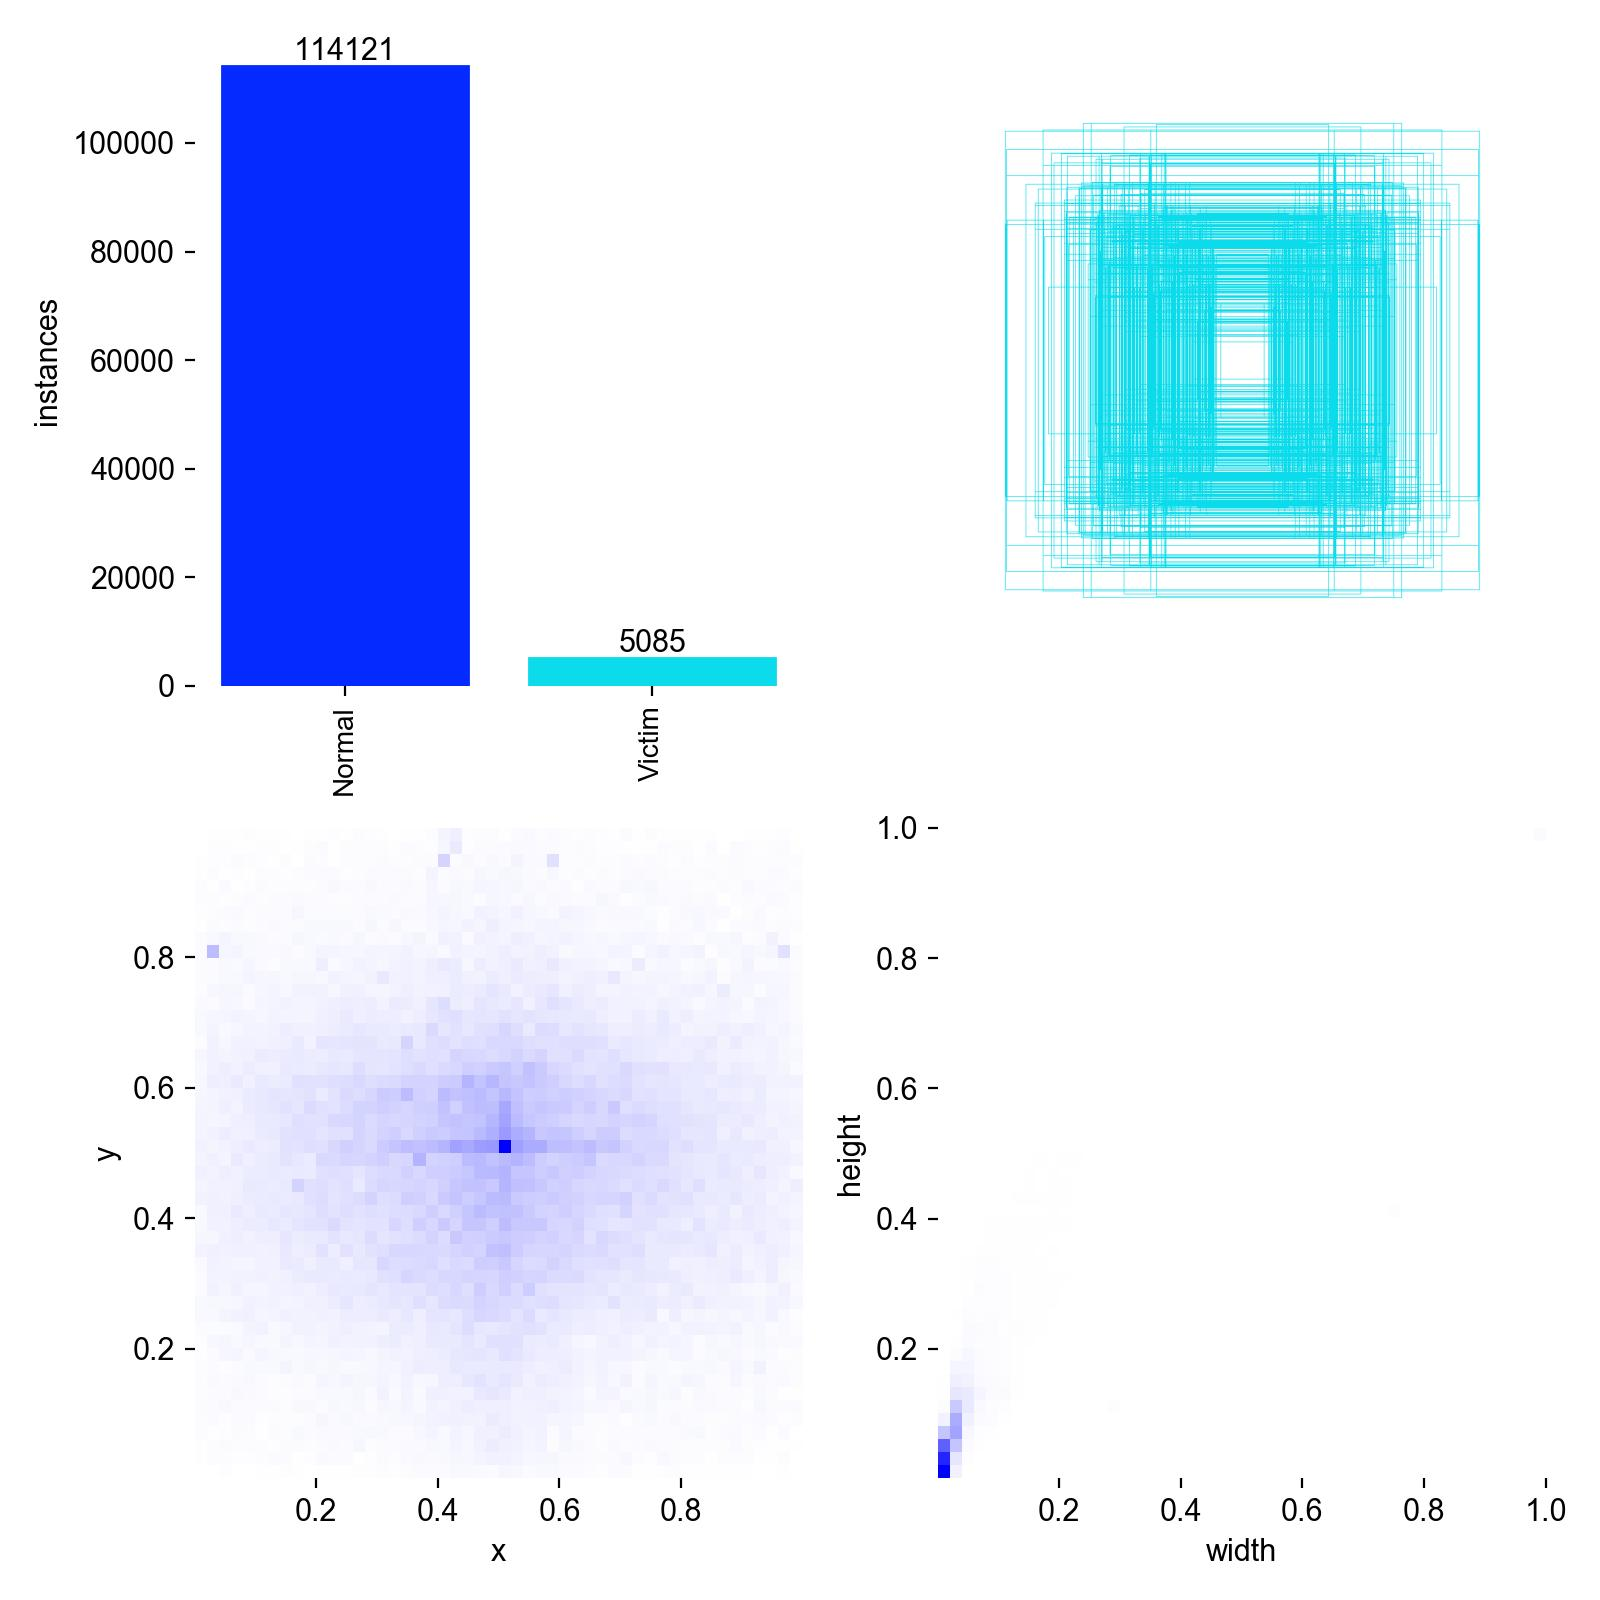
\includegraphics[width=0.65\textwidth]{Images/yolo_ai/rescue_data_dist.jpg}
    \caption[Biểu đồ thống kê phân bổ số lượng khung giới hạn theo lớp Normal và Victim]{\bfseries\fontsize{12pt}{0pt}\selectfont Biểu đồ thống kê phân bổ số lượng khung giới hạn theo lớp Normal và Victim}
    \label{fig:rescue_data_dist}
\end{figure}

Lớp người bình thường (Normal) chiếm tỷ trọng áp đảo tuyệt đối với 114.121 khung giới hạn, trong khi lớp nạn nhân (Victim) chỉ ghi nhận vỏn vẹn 5.085 khung giới hạn (tỷ lệ lệch xấp xỉ 22:1). Đây là thách thức lớn, dễ khiến mô hình học thiên lệch sang lớp đa số.

\paragraph{Đánh giá quá trình hội tụ (Model Convergence):}
Đồ thị tối ưu hóa trọng số của mạng YOLOv8-Rescue qua 50 Epochs chỉ ra mô hình đạt đến trạng thái bão hòa, thể hiện trong Hình \ref{fig:rescue_loss}.

\begin{figure}[H]
    \centering
    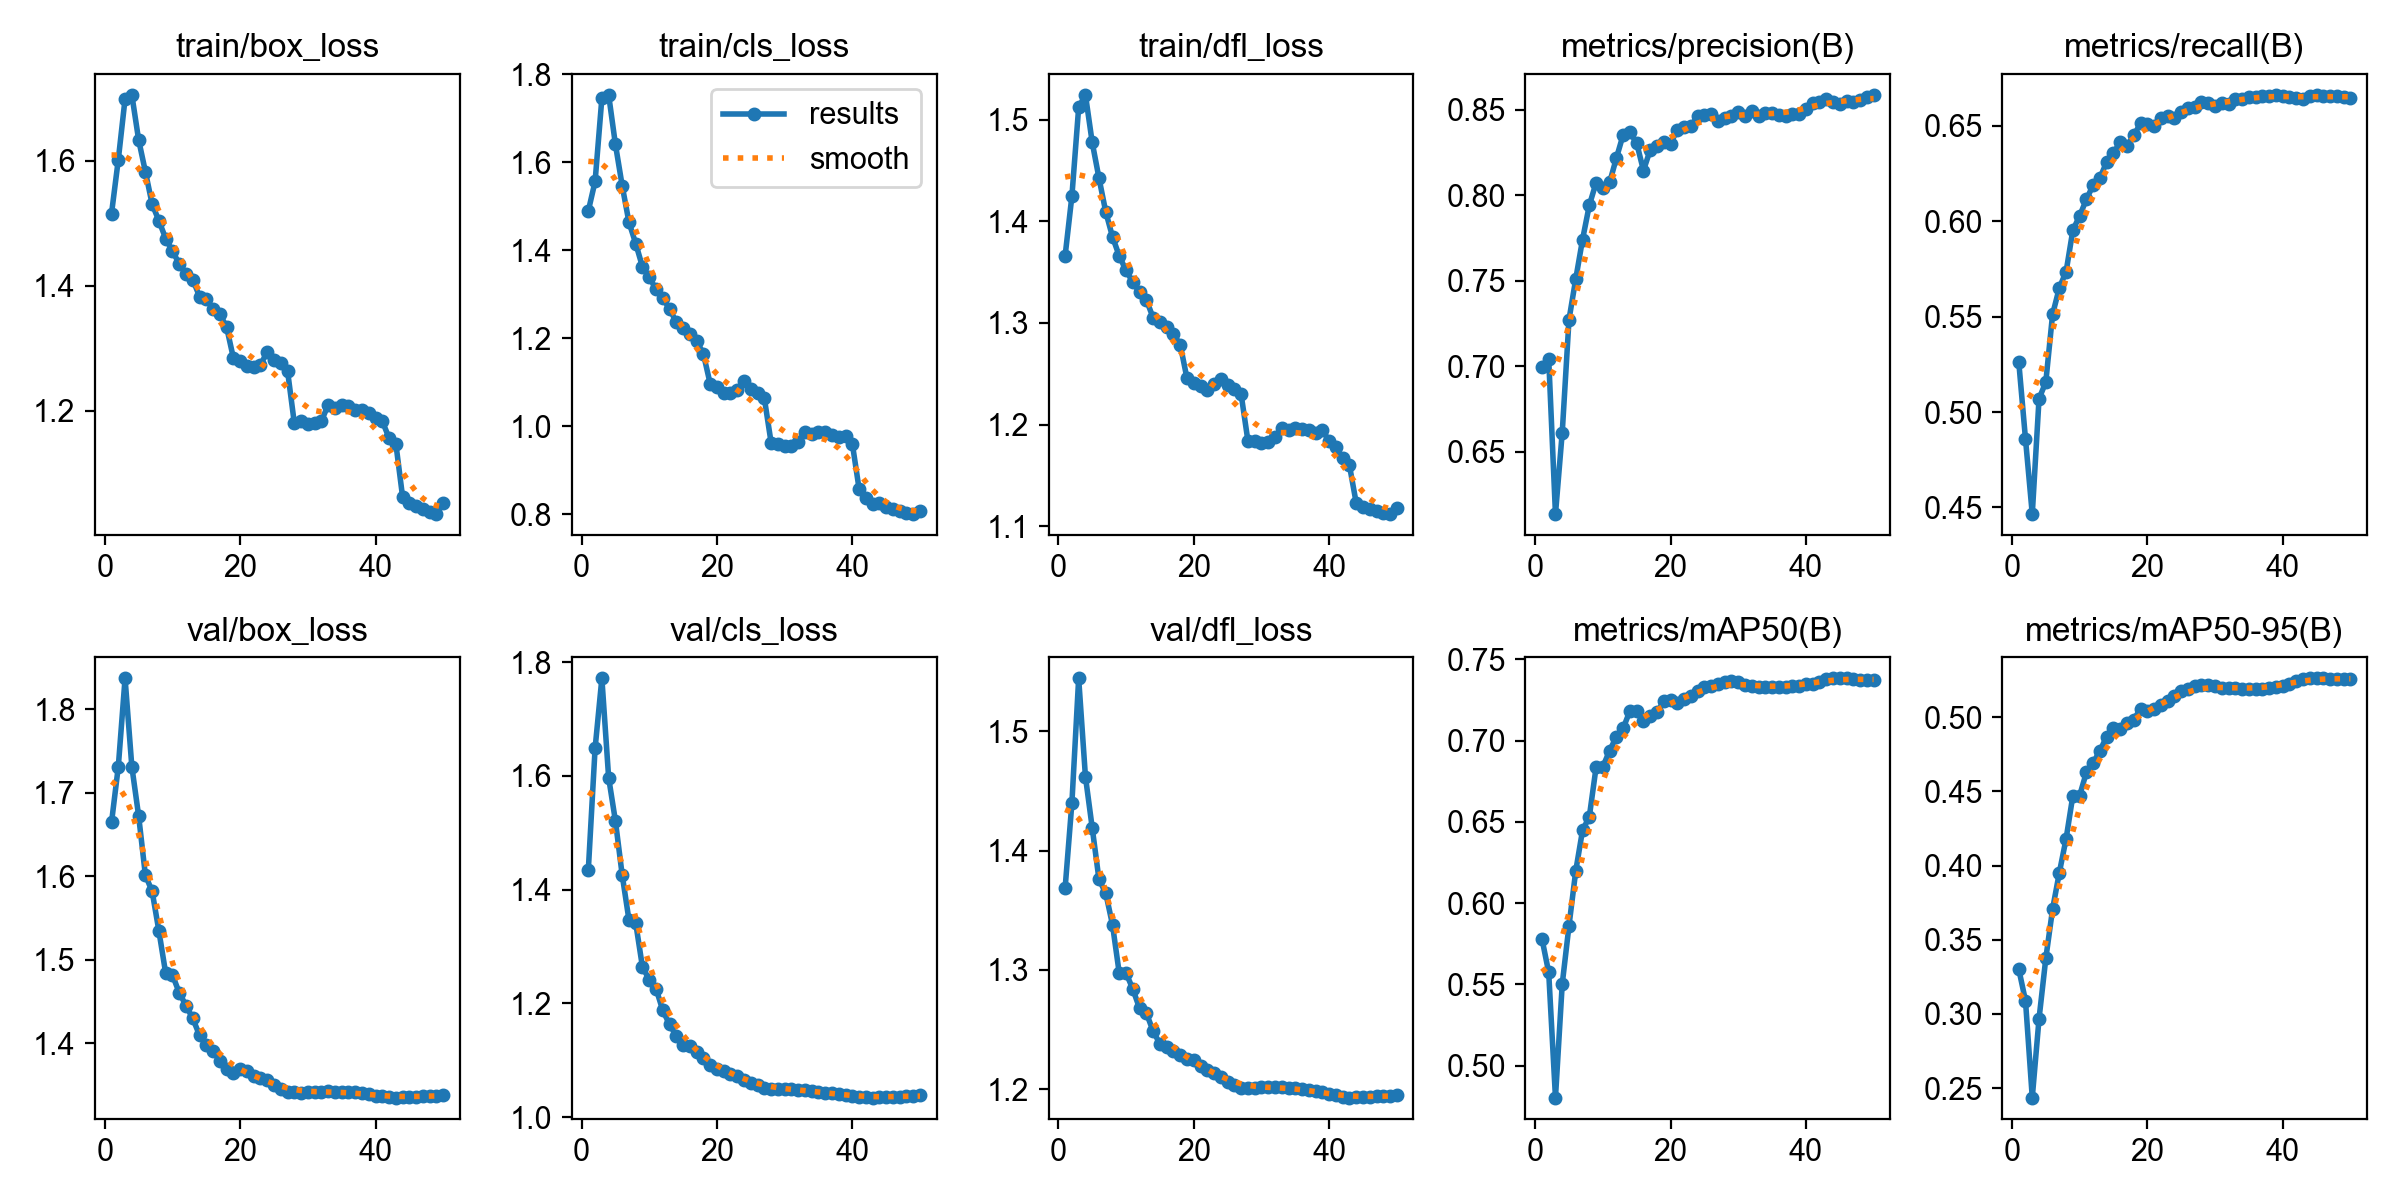
\includegraphics[width=0.75\textwidth]{Images/yolo_ai/rescue_loss.png}
    \caption[Đồ thị biểu diễn hàm suy hao và chỉ số hiệu năng mô hình cứu hộ qua 50 Epochs]{\bfseries\fontsize{12pt}{0pt}\selectfont Đồ thị biểu diễn hàm suy hao và chỉ số hiệu năng mô hình cứu hộ qua 50 Epochs}
    \label{fig:rescue_loss}
\end{figure}

Đường cong hàm suy hao trên tập huấn luyện tiếp tục giảm dần đều đến Epoch 50. Tuy nhiên, trên tập kiểm thử (Validation), đường cong suy hao val/box\_loss và val/cls\_loss bắt đầu đi ngang từ khoảng Epoch 30 đến 40 và không giảm thêm, cho thấy mô hình đã đạt ngưỡng giới hạn hội tụ tối đa với tập dữ liệu hiện hành.

\paragraph{Phân tích hiệu năng tổng thể (Overall Performance):}
Thông số kỹ thuật đánh giá tổng thể cho thấy hệ thống chịu ảnh hưởng nhất định từ sự mất cân bằng dữ liệu đầu vào, thể hiện qua đường F1-Confidence ở Hình \ref{fig:rescue_f1_curve} và Precision-Recall ở Hình \ref{fig:rescue_pr_curve}.

\begin{figure}[H]
    \centering
    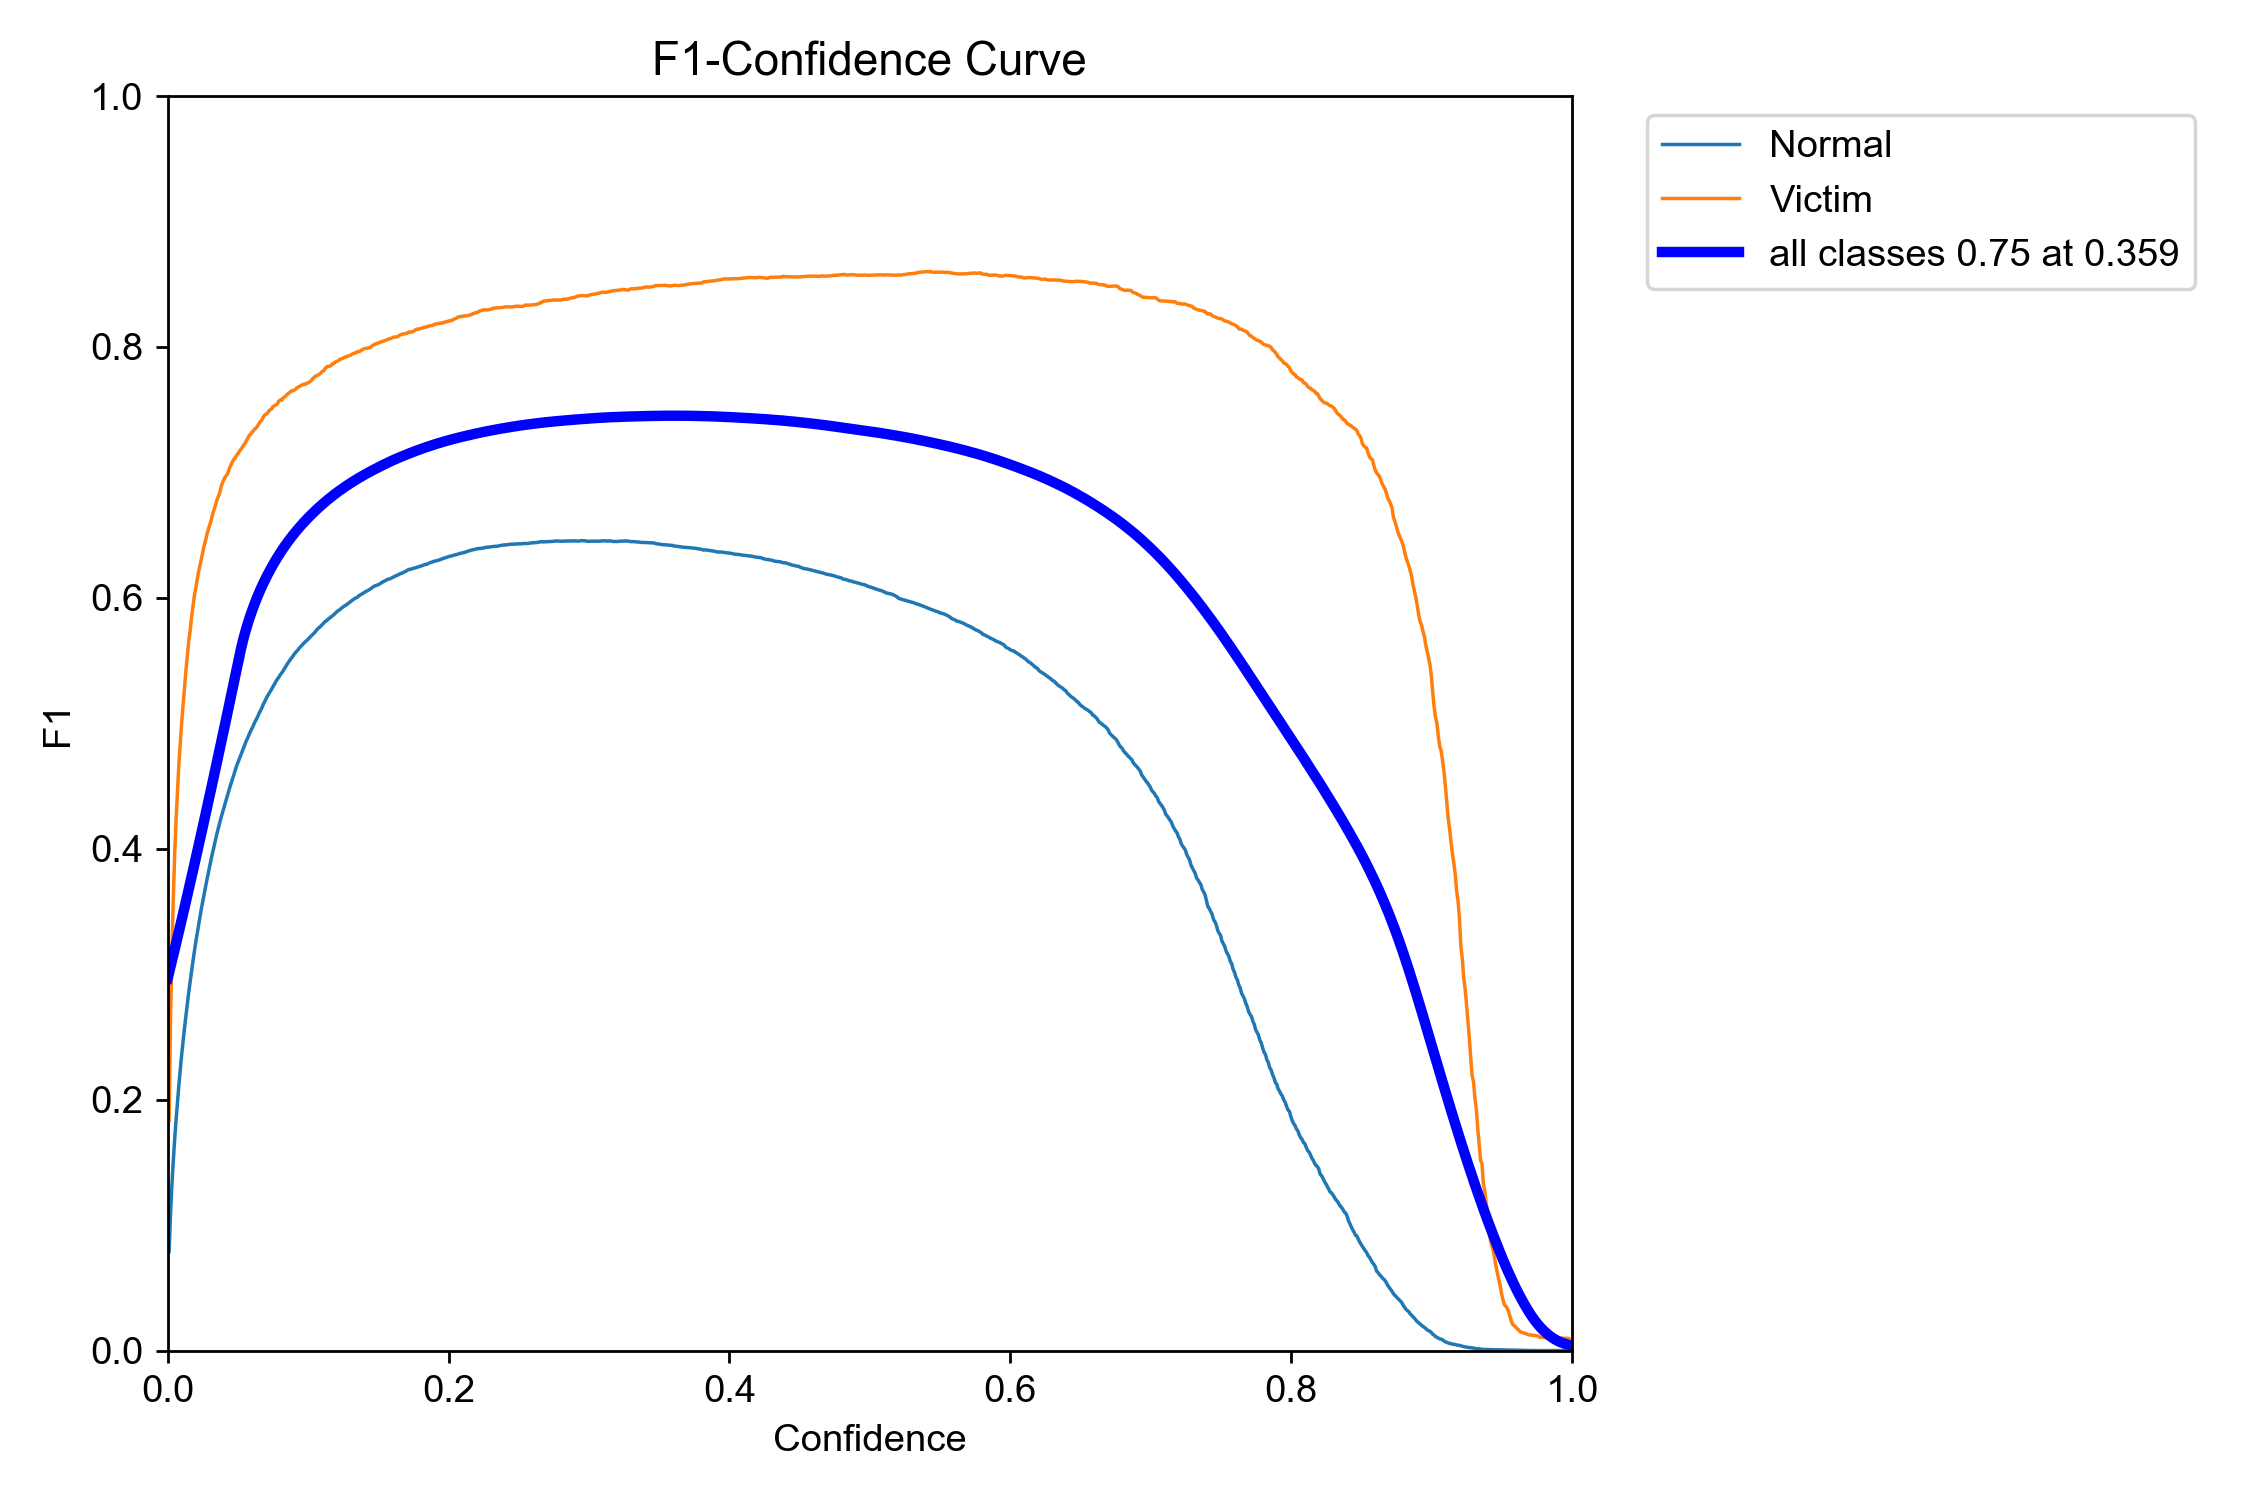
\includegraphics[width=0.65\textwidth]{Images/yolo_ai/rescue_f1_curve.png}
    \caption[Đường cong F1-Confidence đánh giá sự cân bằng của mô hình cứu hộ]{\bfseries\fontsize{12pt}{0pt}\selectfont Đường cong F1-Confidence đánh giá sự cân bằng của mô hình cứu hộ}
    \label{fig:rescue_f1_curve}
\end{figure}

\begin{figure}[H]
    \centering
    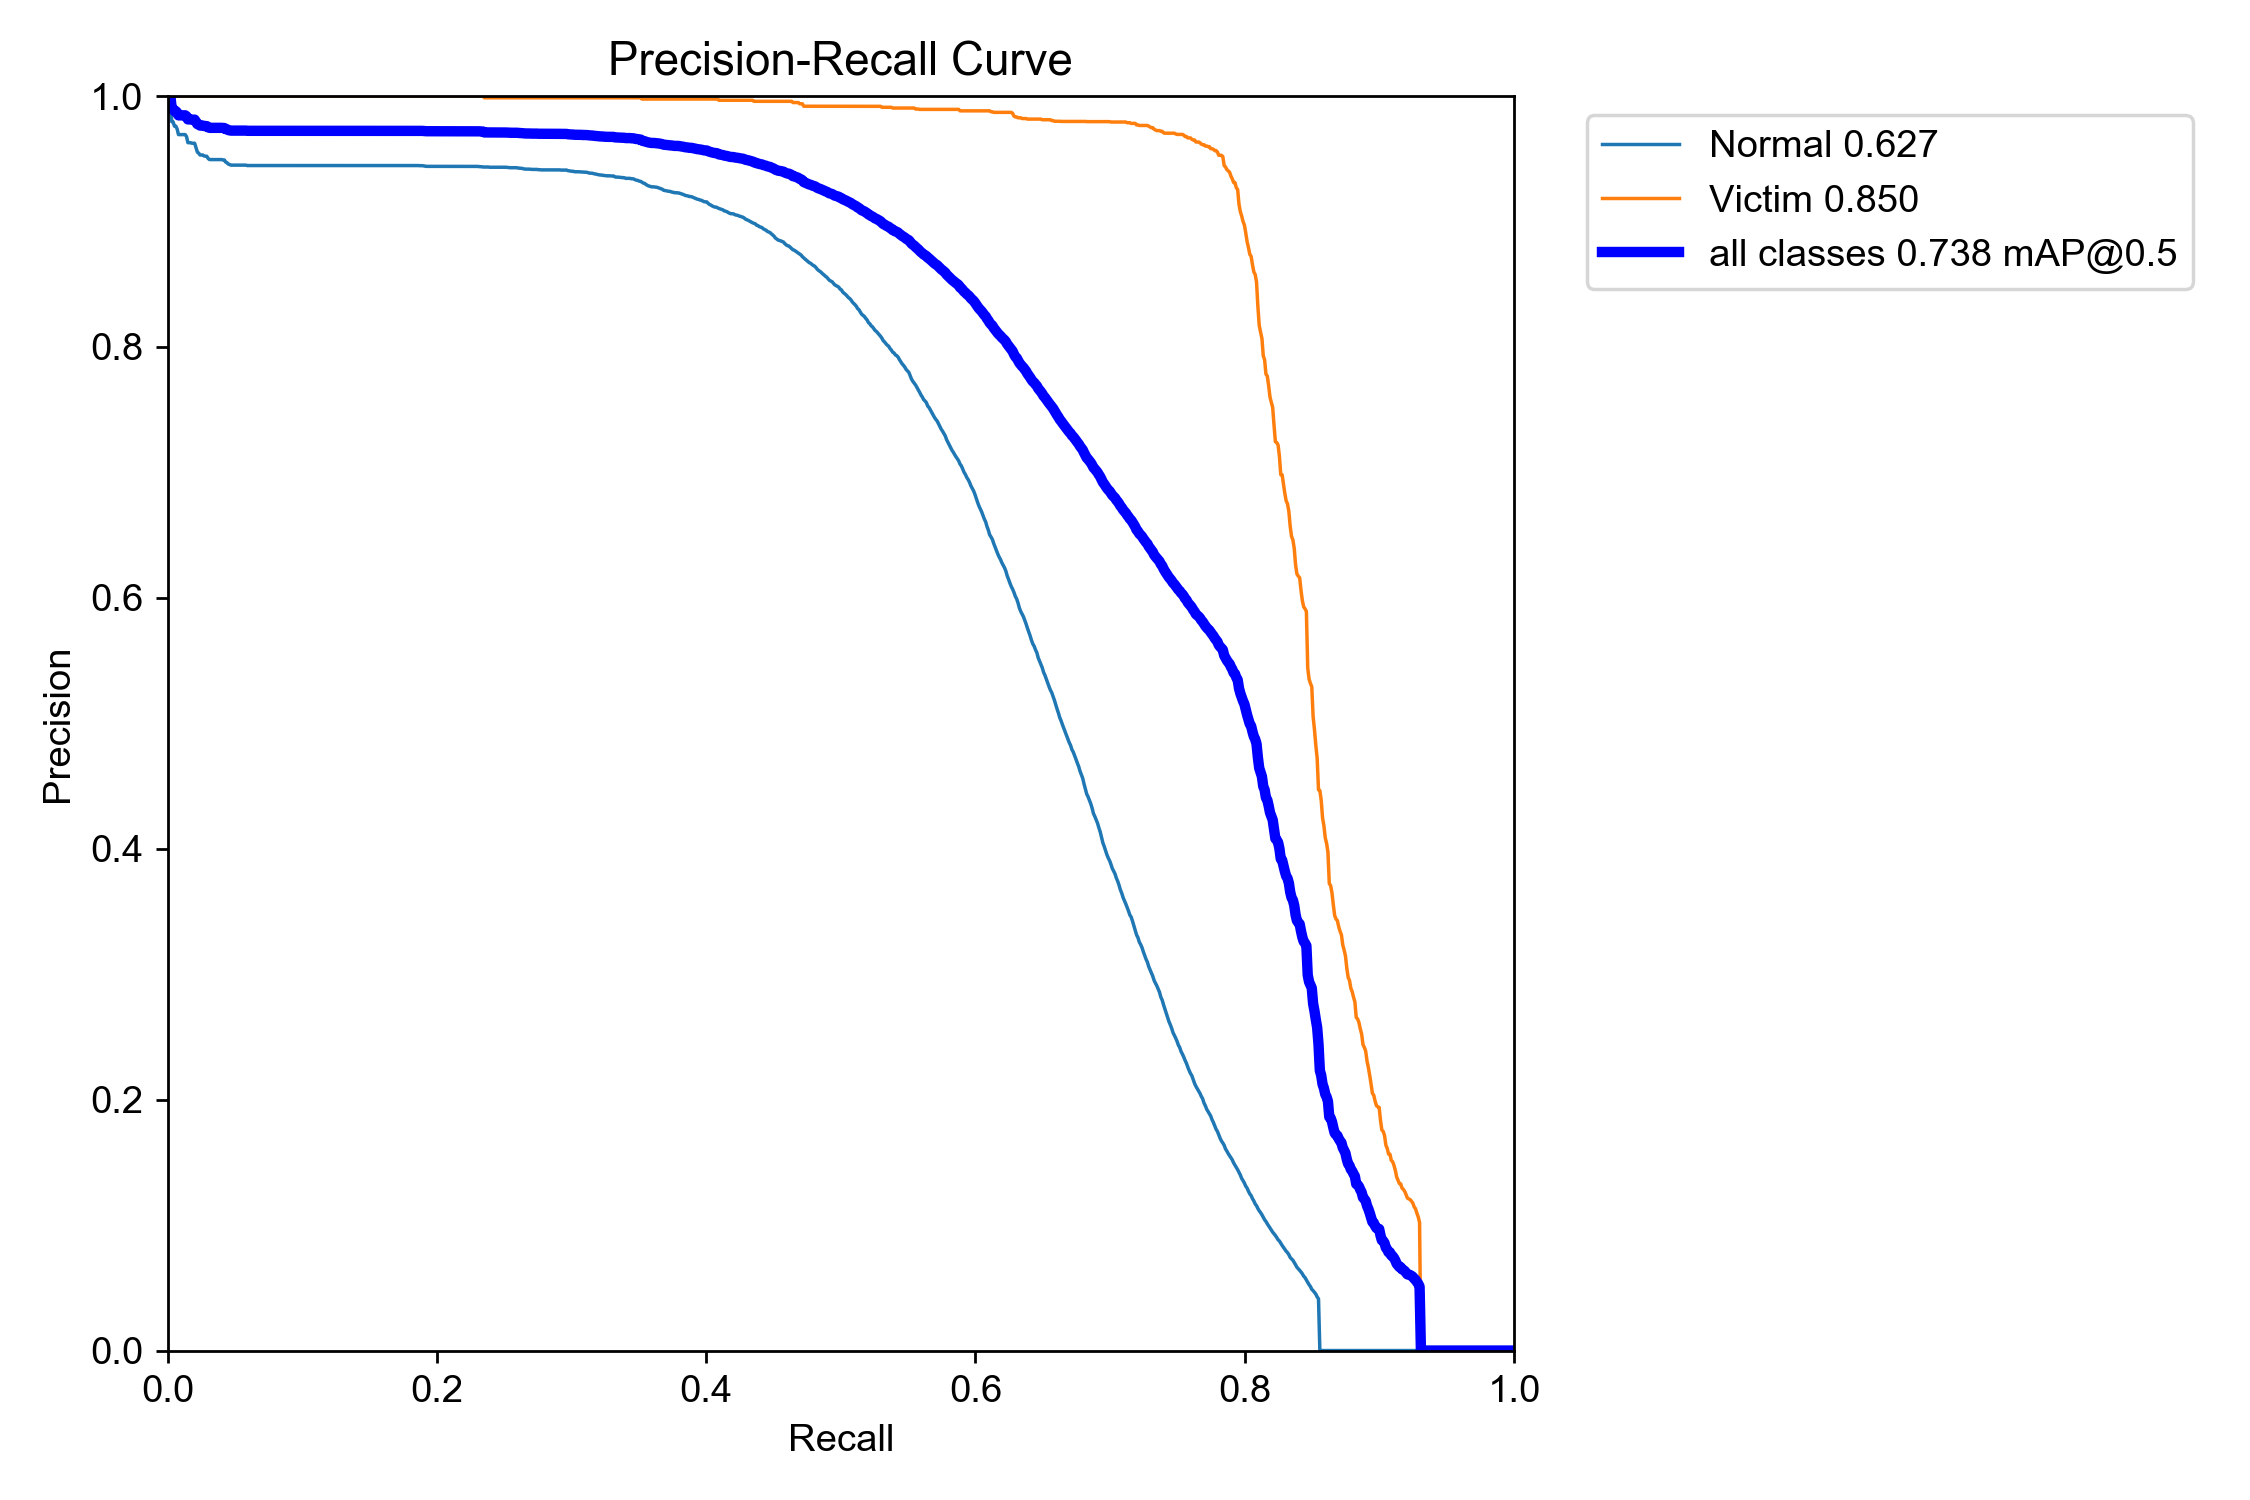
\includegraphics[width=0.65\textwidth]{Images/yolo_ai/rescue_pr_curve.png}
    \caption[Đường cong Precision-Recall của mô hình cứu hộ]{\bfseries\fontsize{12pt}{0pt}\selectfont Đường cong Precision-Recall của mô hình cứu hộ}
    \label{fig:rescue_pr_curve}
\end{figure}

Độ chính xác trung bình toàn cục mAP@0.5 đạt mức 73.8\% (0.738). Hiệu năng ghi nhận sự mất cân đối rõ rệt: lớp Victim đạt mAP@0.5 khá tốt ở mức 85.0\% (0.850), trong khi lớp Normal kéo tụt hiệu năng chung xuống mức mAP@0.5 chỉ đạt 62.7\% (0.627). Chỉ số F1 tổng hợp đạt đỉnh (0.75) khi ngưỡng tin cậy được thiết lập ở mức khá thấp là 0.359.

\paragraph{Đánh giá độ nhạy cảm qua ma trận nhầm lẫn (Confusion Matrix):}
Ma trận nhầm lẫn chuẩn hóa cung cấp cái nhìn chi tiết nhất về các lỗi nhận diện của mô hình cứu hộ, thể hiện ở Hình \ref{fig:rescue_confusion_matrix}.

\begin{figure}[H]
    \centering
    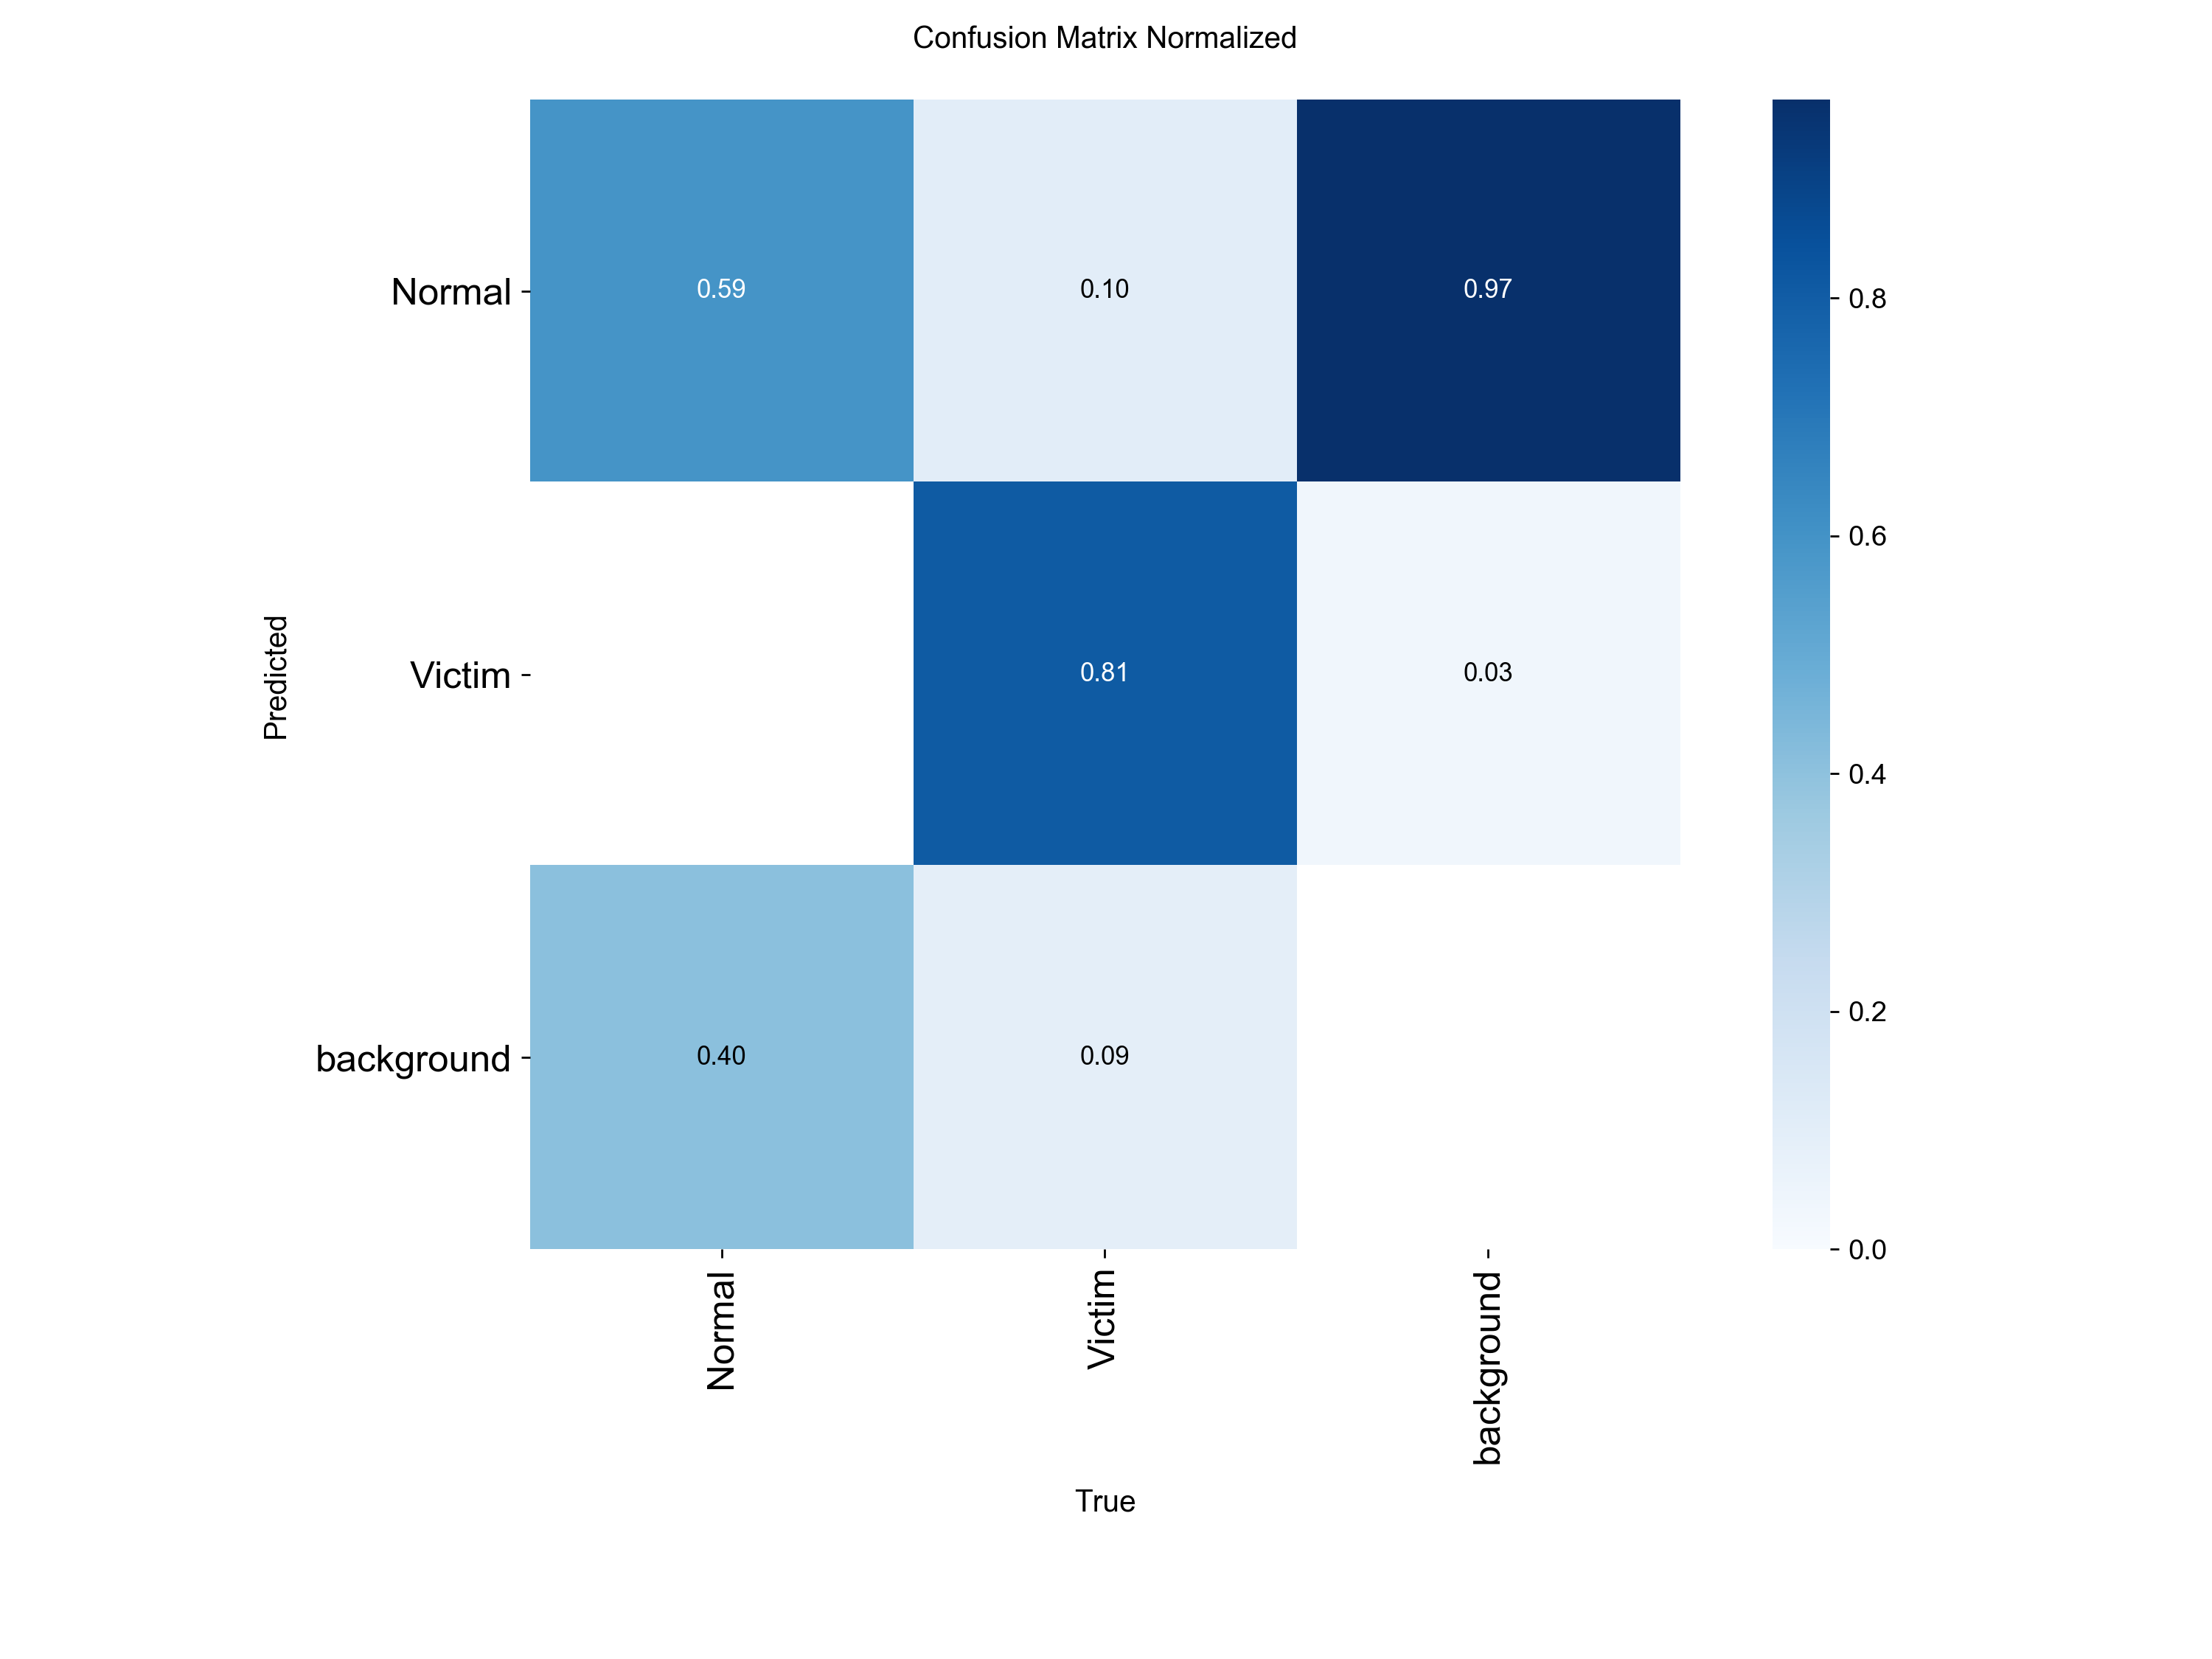
\includegraphics[width=0.6\textwidth]{Images/yolo_ai/rescue_confusion_matrix.png}
    \caption[Ma trận nhầm lẫn chuẩn hóa của mô hình nhận diện cứu hộ]{\bfseries\fontsize{12pt}{0pt}\selectfont Ma trận nhầm lẫn chuẩn hóa của mô hình nhận diện cứu hộ}
    \label{fig:rescue_confusion_matrix}
\end{figure}

Mô hình thực hiện tốt nhiệm vụ ưu tiên khi nhận diện đúng 81\% đối tượng là nạn nhân (Victim). Chỉ có 9\% bị bỏ sót thành cảnh nền và 10\% nhận nhầm thành người bình thường. Tuy nhiên, điểm yếu nằm ở lớp người bình thường (Normal) khi tỷ lệ dự đoán đúng chỉ đạt 59\% và có tới 40\% trường hợp mô hình nhận diện sai các yếu tố nhiễu của môi trường thành người Normal. 

Để khắc phục hạn chế này trong tương lai, giải pháp đề xuất là bổ sung thêm các hình ảnh cảnh nền trống (background images) không chứa người vào tập dữ liệu huấn luyện để mạng nơ-ron học cách phân biệt tốt hơn bối cảnh môi trường.
